\documentclass[12pt,a4paper]{article}

% ---------------- Packages ----------------
\usepackage[a4paper,margin=1in]{geometry}
\usepackage{graphicx}
\usepackage{float}
\usepackage{booktabs}
\usepackage{array}
\usepackage{longtable}
\usepackage{hyperref}
\usepackage{xcolor}
\usepackage{listings}
\usepackage{caption}
\usepackage{titlesec}

% ---------------- Formatting ----------------
\hypersetup{
colorlinks=true,
linkcolor=blue,
urlcolor=blue
}

\setlength{\parindent}{0pt}
\setlength{\parskip}{6pt}

\titleformat{\section}{\Large\bfseries}{\thesection}{1em}{}
\titleformat{\subsection}{\large\bfseries}{\thesubsection}{1em}{}

\lstset{
basicstyle=\ttfamily\small,
breaklines=true,
frame=single,
columns=fullflexible
}

% ---------------- Document ----------------
\begin{document}

% ---------------- Title Page ----------------
\begin{titlepage}
\thispagestyle{empty}
\vspace*{\fill}
\begin{center}
{\Huge\bfseries Self-Driving Dynamic Routing Using OSPF and BGP in the BIRD Routing Stack\par}
\end{center}
\vspace*{\fill}
\end{titlepage}

\tableofcontents
\newpage

% ---------------- Abstract ----------------
\section{Abstract}

This project implements a self-driving dynamic routing lab using the BIRD routing stack. The objective is to demonstrate how modern enterprise networks detect failures, recover automatically, and preserve forwarding during routing control-plane disruptions.

The lab uses OSPF as the intra-domain routing protocol and BGP as the inter-domain/WAN routing protocol. It includes BFD for fast failure detection, OSPF ECMP for path redundancy, NSSA and stub areas for route containment, OSPF area healing across ABRs, and BGP Graceful Restart / Long-Lived Graceful Restart configuration for forwarding continuity during BGP restarts.

The implementation was validated using a multi-router container-based topology. Each experiment includes configuration evidence, measurement logs, packet-loss results, route-table observations, and screenshots. The final validation confirmed that all end-to-end connectivity paths were restored successfully after the experiments.

% ---------------- Project Overview ----------------
\section{Project Overview}

The project proposal required the design and implementation of a self-driving dynamic routing network capable of detecting failures, automatically choosing alternate paths, reducing brownouts, and demonstrating how OSPF and BGP work together in a resilient network.

The implemented lab satisfies this goal using a realistic enterprise-style topology with:

\begin{itemize}
\item OSPF Area 0 as the core backbone.
\item Area Border Routers connecting Area 0 to other areas.
\item NSSA area for controlled external route redistribution.
\item Stub area for branch-style containment.
\item eBGP sessions toward an upstream ISP router.
\item iBGP between internal WAN edge routers.
\item BFD attached to OSPF and BGP sessions.
\item BGP Graceful Restart and Long-Lived Graceful Restart configuration.
\end{itemize}

The project does not simply configure routing protocols. It measures actual behaviour during failures and validates whether the network recovers automatically.

% ---------------- Requirement Mapping ----------------
\section{Proposal Requirement Mapping}

\begin{longtable}{|p{5cm}|p{2.5cm}|p{7cm}|}
\hline
\textbf{Proposal Requirement} & \textbf{Status} & \textbf{Implemented Evidence} \\
\hline
BIRD-based routing lab & Completed & 9-router, 3-host BIRD lab topology. \\
\hline
OSPF Area 0 core & Completed & Core routers configured in Area 0. \\
\hline
ABRs to building/branch areas & Completed & ABR behaviour implemented using hpe-r3 and hpe-r4. \\
\hline
NSSA area & Completed & Area 10 configured as NSSA. \\
\hline
Stub area & Completed & Area 20 configured as stub area. \\
\hline
eBGP to ISP/upstream & Completed & hpe-r1/hpe-r2 peer with hpe-r9. \\
\hline
iBGP internally & Completed & hpe-r1 and hpe-r2 internal BGP session. \\
\hline
BFD attached to BGP & Completed & BGP WAN edge failure detected using BFD. \\
\hline
BFD attached to OSPF & Completed & OSPF-BFD sessions enabled and tested. \\
\hline
BFD single-hop detection below 300 ms & Completed & BFD WAN detection measured at 61 ms. \\
\hline
OSPF failure recovery & Completed & OSPF core link failure recovery measured. \\
\hline
OSPF ECMP failover & Completed & Native OSPF ECMP and OSPF-BFD assisted ECMP measured. \\
\hline
NSSA Type-7 / Type-5 behaviour & Completed & Type-7 inside NSSA and Type-5 outside NSSA observed. \\
\hline
OSPF area healing across ABRs & Completed & Area 10 to Area 20 recovery tested after ABR link failure. \\
\hline
BGP Graceful Restart & Completed & Forwarding continuity observed during BGP control-plane restart. \\
\hline
LLGR configuration & Completed & Long-lived graceful restart configured with LL stale time. \\
\hline
Route withdrawal behaviour & Completed & Real route withdrawal caused route removal and packet loss. \\
\hline
Topology diagram & Completed & Topology documented in Markdown, Mermaid, and LaTeX. \\
\hline
Before/after configurations & Completed & Config snapshots and modified configs stored. \\
\hline
Measurement logs & Completed & CSVs, evidence logs, route samples, and ping logs saved. \\
\hline
Screenshots & Completed & Screenshots collected for all major experiments. \\
\hline
Graphs & Pending / Optional & CSV results are available; graphs can be generated as final polish. \\
\hline
BIRD source-code patch & Not in scope & This was an excellence-level optional item, not required for minimum delivery. \\
\hline
\end{longtable}

% ---------------- Topology ----------------
\section{Lab Topology}

\subsection{Objective}

The lab topology was designed to emulate a small enterprise network using the BIRD routing stack. The topology includes an OSPF campus core, non-backbone OSPF areas, WAN edge routers, an upstream ISP router, internal hosts, eBGP, iBGP, BFD, and BGP Graceful Restart mechanisms.

The purpose of this topology is to provide a realistic environment for testing self-healing routing behaviour under link failures, control-plane restarts, and routing convergence events.

\subsection{Topology Overview}

The topology contains nine routers and three end hosts. Routers hpe-r1, hpe-r2, hpe-r3, and hpe-r4 form the enterprise OSPF Area 0 core. Routers hpe-r3 and hpe-r4 act as Area Border Routers. Router hpe-r3 connects the core to the NSSA-style Area 10, while router hpe-r4 connects the core to the stub-style Area 20.

The external ISP or upstream network is represented by hpe-r9. The enterprise edge routers hpe-r1 and hpe-r2 connect to hpe-r9 using eBGP. The two enterprise edge routers also exchange routes internally using iBGP.

\subsection{Router Roles}

\begin{table}[h]
\centering
\begin{tabular}{|l|p{9cm}|}
\hline
\textbf{Node} & \textbf{Role} \\
\hline
hpe-r1 & Enterprise WAN edge router, OSPF Area 0 router, eBGP peer with hpe-r9, and iBGP peer with hpe-r2. \\
\hline
hpe-r2 & Enterprise WAN edge router, OSPF Area 0 router, eBGP peer with hpe-r9, and iBGP peer with hpe-r1. \\
\hline
hpe-r3 & Area Border Router between OSPF Area 0 and NSSA Area 10. \\
\hline
hpe-r4 & Area Border Router between OSPF Area 0 and Stub Area 20. \\
\hline
hpe-r5 & Internal router inside NSSA Area 10. \\
\hline
hpe-r6 & NSSA branch gateway router for host hpe-h1. \\
\hline
hpe-r7 & Internal router inside Stub Area 20. \\
\hline
hpe-r8 & Stub branch gateway router for host hpe-h2. \\
\hline
hpe-r9 & External ISP/upstream router in AS65002 and gateway for hpe-h3. \\
\hline
\end{tabular}
\caption{Router roles in the BIRD routing lab}
\end{table}

\subsection{Host Networks}

\begin{table}[h]
\centering
\begin{tabular}{|l|l|l|}
\hline
\textbf{Host} & \textbf{IP Address} & \textbf{Gateway Router} \\
\hline
hpe-h1 & 10.0.61.2/24 & hpe-r6 \\
\hline
hpe-h2 & 10.0.82.2/24 & hpe-r8 \\
\hline
hpe-h3 & 10.0.93.2/24 & hpe-r9 \\
\hline
\end{tabular}
\caption{End-host addressing used in the lab}
\end{table}

\subsection{Routing Design}

OSPF is used as the internal routing protocol. Area 0 represents the campus or headquarters core. Area 10 is used as an NSSA-style branch or guest area, and Area 20 is used as a stub-style branch area. This allows the lab to demonstrate area-based containment and ABR-based healing.

BGP is used for WAN and inter-domain routing. Routers hpe-r1 and hpe-r2 peer with hpe-r9 using eBGP, while hpe-r1 and hpe-r2 also exchange routes internally using iBGP. BGP Graceful Restart and Long-Lived Graceful Restart are configured for later control-plane recovery experiments.

BFD is enabled on WAN-edge BGP sessions to provide fast failure detection. This allows the lab to test sub-second detection and recovery behaviour on edge links.

\subsection{Conclusion}

The topology provides a realistic small-scale enterprise routing environment. It contains an OSPF core, ABRs, NSSA and stub areas, eBGP WAN connectivity, iBGP internal routing, BFD-based fast failure detection, and BGP state-preservation mechanisms. This makes it suitable for testing the self-healing routing mechanisms required by the project.



\begin{figure}[H]
\centering

\includegraphics[width=0.95\textwidth]{figures/topology.png}
\caption{Implemented BIRD routing lab topology}
\end{figure}


% ---------------- Tools and Environment ----------------
\section{Tools and Environment}

The project was implemented using a Linux-based container lab.

The main tools used were:

\begin{itemize}
\item Linux networking namespaces / containers
\item BIRD routing daemon
\item BFD inside BIRD
\item OSPF and BGP protocol configuration
\item Bash scripts for automated experiments
\item Python scripts for parsing logs and generating CSV results
\item ping for traffic continuity measurement
\item ip route and birdc commands for route observation
\item Mermaid / LaTeX for documentation
\end{itemize}

The lab contains routers \texttt{hpe-r1} to \texttt{hpe-r9} and hosts \texttt{hpe-h1}, \texttt{hpe-h2}, and \texttt{hpe-h3}.

% ---------------- Baseline ----------------
\section{Baseline Validation}

\subsection{Objective}

The objective of the baseline validation was to confirm that the routing lab was healthy before running failure experiments.

A stable baseline is important because convergence and failover results are meaningful only when the network starts from a known working state.

\subsection{Validated Conditions}

The baseline validation checked the following conditions:

\begin{itemize}
    \item All HPE router and host containers were running.
    \item BIRD was running on all routers.
    \item OSPF was running.
    \item OSPF neighbours were in the Full state.
    \item BGP sessions were Established.
    \item BFD sessions on the WAN edge were Up.
    \item End-to-end host connectivity worked with zero packet loss.
\end{itemize}

\subsection{Baseline Connectivity Results}

\begin{table}[h]
\centering
\begin{tabular}{|l|l|l|l|}
\hline
\textbf{Test} & \textbf{Source} & \textbf{Destination} & \textbf{Packet Loss} \\
\hline
h1\_to\_h2 & hpe-h1 & 10.0.82.2 & 0\% \\
h2\_to\_h1 & hpe-h2 & 10.0.61.2 & 0\% \\
h1\_to\_h3 & hpe-h1 & 10.0.93.2 & 0\% \\
h2\_to\_h3 & hpe-h2 & 10.0.93.2 & 0\% \\
h3\_to\_h1 & hpe-h3 & 10.0.61.2 & 0\% \\
h3\_to\_h2 & hpe-h3 & 10.0.82.2 & 0\% \\
\hline
\end{tabular}
\caption{Baseline end-to-end connectivity results}
\end{table}

\subsection{Conclusion}

The baseline validation confirmed that the lab was stable before failure testing. OSPF was running with Full neighbour adjacencies, BGP sessions were Established, BFD sessions were Up on the WAN edge, and all host-to-host connectivity tests completed with zero packet loss.

This baseline is the reference state for later BFD, OSPF, ECMP, and BGP GR/LLGR experiments.


% ---------------- Config Snapshot ----------------
\section{Configuration Snapshot}

\subsection{Objective}

The objective of this deliverable was to save a clean baseline snapshot of the working lab configuration.

This snapshot was taken after baseline validation confirmed that containers were running, OSPF neighbours were in the Full state, BGP sessions were Established, BFD sessions were Up, and end-to-end host connectivity worked with zero packet loss.

\subsection{Captured Files}

The snapshot includes the following files:

\begin{itemize}
    \item BIRD configuration from each router.
    \item Runtime state from each router.
    \item Runtime state from each host.
    \item A manifest describing the snapshot contents.
\end{itemize}

\subsection{Snapshot Location}

The timestamped baseline snapshot is stored in:

\begin{verbatim}
configs/baseline/20260623_142648/
\end{verbatim}

The latest baseline snapshot is also available in:

\begin{verbatim}
configs/baseline/latest/
\end{verbatim}

\subsection{Importance}

The project proposal requires configuration evidence before and after tuning. This snapshot acts as the baseline configuration state before additional experiments such as BFD tuning, OSPF healing, ECMP failover, and BGP GR/LLGR testing.

\subsection{Conclusion}

The baseline configuration snapshot was successfully created. It provides a reproducible reference point for comparing future tuned configurations and experiment results.


% ---------------- BFD ----------------
\section{BFD WAN Edge Failure Detection}

\subsection{Objective}

The objective of this experiment was to validate fast failure detection on the WAN edge using Bidirectional Forwarding Detection, or BFD.

The tested failure was the WAN edge link between \texttt{hpe-r2} and \texttt{hpe-r9}. This link carries eBGP between the enterprise edge router and the upstream ISP router. BFD was attached to the BGP session so that link or session failure could be detected quickly.

\subsection{Test Setup}

\begin{table}[h]
\centering
\begin{tabular}{|l|l|}
\hline
\textbf{Item} & \textbf{Value} \\
\hline
Failed router & hpe-r2 \\
\hline
Failed interface & eth1 \\
\hline
Failed peer & hpe-r9 \\
\hline
BFD peer IP & 10.0.29.3 \\
\hline
Traffic source & hpe-h1 \\
\hline
Traffic destination & hpe-h3 \\
\hline
Destination IP & 10.0.93.2 \\
\hline
\end{tabular}
\caption{BFD WAN edge failure test setup}
\end{table}

\subsection{BFD Timer Configuration}

The observed BFD session timing values were:

\begin{table}[h]
\centering
\begin{tabular}{|l|l|}
\hline
\textbf{Field} & \textbf{Value} \\
\hline
BFD interval & 0.100 seconds \\
\hline
BFD timeout & 0.500 seconds \\
\hline
\end{tabular}
\caption{Observed BFD timing values}
\end{table}

\subsection{Measurement Result}

The BFD WAN edge failure experiment measured how quickly the network detected the failure of the direct WAN edge path between \texttt{hpe-r2} and \texttt{hpe-r9}. The failed BFD peer was \texttt{10.0.29.3}. During the test, traffic was continuously sent from \texttt{hpe-h1} to \texttt{hpe-h3}.

\begin{table}[H]
\centering
\small
\renewcommand{\arraystretch}{1.25}
\begin{tabular}{|p{6cm}|p{5cm}|}
\hline
\textbf{Measurement} & \textbf{Result} \\
\hline
Failed router & \texttt{hpe-r2} \\
\hline
Failed interface & \texttt{eth1} \\
\hline
Failed BFD peer & \texttt{10.0.29.3} \\
\hline
Traffic source & \texttt{hpe-h1} \\
\hline
Traffic destination & \texttt{hpe-h3} \\
\hline
Destination IP & \texttt{10.0.93.2} \\
\hline
BFD detection time & 61 ms \\
\hline
BGP reaction time & 61 ms \\
\hline
Packets transmitted & 293 \\
\hline
Packets received & 293 \\
\hline
Packets lost & 0 \\
\hline
Packet loss & 0.00\% \\
\hline
Alternate path after failure & \texttt{hpe-r2 -> hpe-r1 -> hpe-r9} \\
\hline
\end{tabular}
\caption{BFD WAN edge failure detection measurement result}
\end{table}

The project target for single-hop BFD failure detection was below 300 ms. The measured detection time was 61 ms, so the experiment successfully satisfies the target. The ping result also shows that traffic continued with 0.00\% packet loss.

\begin{table}[h]
\centering
\begin{tabular}{|l|l|}
\hline
\textbf{Metric} & \textbf{Result} \\
\hline
BFD detection time & 61 ms \\
\hline
BGP reaction time & 61 ms \\
\hline
Estimated packets transmitted & 293 \\
\hline
Packets received & 293 \\
\hline
Lost packets & 0 \\
\hline
Packet loss & 0.00\% \\
\hline
Explicit unreachable packets & 0 \\
\hline
\end{tabular}
\caption{BFD WAN edge failure measurement result}
\end{table}

\subsection{Path Before Failure}

Before the failure, \texttt{hpe-r2} reached the external host network through the direct WAN edge link to \texttt{hpe-r9}.

\begin{verbatim}
10.0.93.2 via 10.0.29.3 dev eth1
\end{verbatim}

This means the original forwarding path was:

\begin{verbatim}
hpe-r2 -> hpe-r9
\end{verbatim}

\subsection{Path During Failure}

After the \texttt{hpe-r2} to \texttt{hpe-r9} link was brought down, BFD detected the failure and BGP removed the failed direct route. During the failure, \texttt{hpe-r2} changed its route to the external network through \texttt{hpe-r1}.

\begin{verbatim}
10.0.93.2 via 10.0.12.2 dev eth2
\end{verbatim}

At the same time, \texttt{hpe-r1} still had reachability to the ISP router through its own WAN edge link.

\begin{verbatim}
10.0.93.2 via 10.0.19.3 dev eth0
\end{verbatim}

Therefore, the alternate forwarding path became:

\begin{verbatim}
hpe-r2 -> hpe-r1 -> hpe-r9
\end{verbatim}

\subsection{Traffic Behaviour During Failure}

During the failure window, traffic from \texttt{hpe-h1} to \texttt{hpe-h3} remained successful.

\begin{verbatim}
10 packets transmitted, 10 received, 0\% packet loss
\end{verbatim}

The longer timestamped ping monitor also showed:

\begin{verbatim}
293 packets transmitted, 293 received, 0 lost, 0.00\% packet loss
\end{verbatim}

\subsection{Restore Behaviour}

After the failed link was restored, BFD became Up again on both sides. The BGP session between \texttt{hpe-r2} and \texttt{hpe-r9} also returned to Established state after a short reconnection period.

The final restore confirmation showed that direct link pings worked, BFD was Up, BGP was Established, and end-to-end traffic from \texttt{hpe-h1} to \texttt{hpe-h3} worked with zero packet loss.



\subsection{Conclusion}

The BFD WAN edge failure experiment successfully demonstrated fast failure detection and automatic routing recovery.

BFD detected the \texttt{hpe-r2} to \texttt{hpe-r9} WAN edge failure in 61 ms. BGP reacted in the same 61 ms window. After the failed direct path was removed, traffic shifted to the alternate path through \texttt{hpe-r1} and continued toward \texttt{hpe-r9}.

The traffic test showed 0.00\% packet loss during the failure window. After link restoration, BFD and BGP recovered cleanly. This confirms that BFD can provide sub-second WAN failure detection and help maintain reachability through alternate paths.

\section{Multi-hop BFD Failure Detection}

\subsection{Purpose}

The earlier BFD experiments used directly connected BFD peers. In this experiment, a multi-hop BFD session was configured between \texttt{hpe-r1} and \texttt{hpe-r8}. These routers are not directly connected, so BFD packets travel through the routed OSPF network.

The goal of this experiment was to verify whether BFD can detect failure of a routed multi-hop path within the project target of less than 1 second.

\subsection{Multi-hop BFD Endpoints}

The multi-hop BFD session used the following endpoints:

\begin{table}[H]
\centering
\small
\renewcommand{\arraystretch}{1.25}
\begin{tabular}{|p{5cm}|p{6cm}|}
\hline
\textbf{Router} & \textbf{Multi-hop BFD Peer} \\
\hline
\texttt{hpe-r1} & \texttt{10.0.82.3} \\
\hline
\texttt{hpe-r8} & \texttt{10.0.14.2} \\
\hline
\end{tabular}
\caption{Multi-hop BFD endpoints}
\end{table}

Before failure, the BFD session was observed in the \texttt{Up} state on both routers. The interface column showed \texttt{---}, confirming that the session was not tied to a directly connected interface.

\subsection{Failure Scenario}

The routed path between the two BFD endpoints used the branch-side path through \texttt{hpe-r4} and \texttt{hpe-r7}. To trigger a multi-hop reachability failure, the interface \texttt{eth2} on \texttt{hpe-r4} was brought down.

\begin{verbatim}
docker exec hpe-r4 ip link set eth2 down
\end{verbatim}

This broke the path:

\begin{verbatim}
hpe-r1 -> hpe-r4 -> hpe-r7 -> hpe-r8
\end{verbatim}

\subsection{Measurement Result}

\begin{table}[H]
\centering
\small
\renewcommand{\arraystretch}{1.25}
\begin{tabular}{|p{6cm}|p{5cm}|}
\hline
\textbf{Measurement} & \textbf{Result} \\
\hline
Failed link & \texttt{hpe-r4 eth2} to \texttt{hpe-r7 eth1} \\
\hline
\texttt{hpe-r1} BFD detection time & 546 ms \\
\hline
\texttt{hpe-r8} BFD detection time & 629 ms \\
\hline
\texttt{hpe-r1} BFD recovery time & 7645 ms \\
\hline
\texttt{hpe-r8} BFD recovery time & 2 ms \\
\hline
Ping packets transmitted & 269 \\
\hline
Ping packets received & 79 \\
\hline
Ping loss & 70.632\% \\
\hline
Target below 1 second & Yes \\
\hline
\end{tabular}
\caption{Multi-hop BFD failure detection result}
\end{table}

The measured multi-hop BFD failure detection times were 546 ms on \texttt{hpe-r1} and 629 ms on \texttt{hpe-r8}. Both values are below the 1-second target.

The packet loss is high because the experiment intentionally broke the routed path between the multi-hop BFD endpoints. This test mainly validates fast multi-hop failure detection, not traffic failover.

\subsection{Conclusion}

This experiment satisfies the multi-hop BFD deliverable. It proves that BIRD can run BFD between non-directly connected routers and detect routed-path failure in sub-second time.


% ---------------- OSPF Core Failure ----------------
\section{OSPF Core Link Failure Recovery}

\subsection{Objective}

The objective of this experiment was to validate OSPF fast recovery when an internal core link fails.

The tested failure was the core OSPF link between \texttt{hpe-r3} and \texttt{hpe-r2}. The goal was to observe whether OSPF could detect the failure, remove the failed path, install an alternate path, and restore forwarding quickly.

\subsection{Test Setup}

\begin{table}[h]
\centering
\begin{tabular}{|l|l|}
\hline
\textbf{Item} & \textbf{Value} \\
\hline
Failed router & hpe-r3 \\
\hline
Failed core peer & hpe-r2 \\
\hline
Old next-hop & 10.0.23.2 \\
\hline
New next-hop & 10.0.13.2 \\
\hline
Test type & OSPF core link failure \\
\hline
Primary measurement method & Linux kernel route monitor \\
\hline
Supporting methods & ip route get and BIRD route sampling \\
\hline
Traffic measurement & Timestamped ICMP ping \\
\hline
\end{tabular}
\caption{OSPF core link failure test setup}
\end{table}

\subsection{Measurement Method}

OSPF convergence is not only a control-plane event. A route may change inside BIRD first, but traffic is forwarded by the Linux kernel routing table.

Because of this, three different measurement methods were used. The Linux kernel route monitor was treated as the primary convergence measurement because it shows when the actual forwarding route changed in the kernel. The \texttt{ip route get} and BIRD route-table samples were used as supporting confirmation.

\subsection{Measurement Result}

\begin{table}[h]
\centering
\begin{tabular}{|l|l|}
\hline
\textbf{Metric} & \textbf{Result} \\
\hline
Old next-hop & 10.0.23.2 \\
\hline
New next-hop & 10.0.13.2 \\
\hline
Kernel route monitor convergence time & 628 ms \\
\hline
ip route get sample convergence time & 631 ms \\
\hline
BIRD route-table sample convergence time & 648 ms \\
\hline
Estimated transmitted packets & 350 \\
\hline
Received packets & 338 \\
\hline
Failed/lost packets & 12 \\
\hline
Estimated packet loss & 3.43\% \\
\hline
Explicit unreachable packets & 1 \\
\hline
\end{tabular}
\caption{OSPF core link failure measurement result}
\end{table}

\subsection{Path Change}

Before the failure, the route used the old next-hop:

\begin{verbatim}
10.0.23.2
\end{verbatim}

After the core link failure, OSPF selected the alternate next-hop:

\begin{verbatim}
10.0.13.2
\end{verbatim}

This means OSPF successfully removed the failed path and installed an alternate route.

\subsection{Convergence Analysis}

The three convergence measurements were close:

\begin{verbatim}
Kernel route monitor: 628 ms
ip route get sampling: 631 ms
BIRD route sampling: 648 ms
\end{verbatim}

This consistency shows that the result is reliable. The kernel forwarding table changed first at around 628 ms, and the supporting measurements confirmed the same route transition within a small time gap.

\subsection{Traffic Impact}

The ping log did not contain a normal final ping summary, so packet loss was estimated using ICMP sequence numbers.

The parsed result was:

\begin{verbatim}
Estimated transmitted packets: 350
Received packets: 338
Failed/lost packets: 12
Estimated packet loss percent: 3.43\%
Explicit unreachable packets seen: 1
\end{verbatim}

This shows that traffic experienced a short disruption during OSPF reconvergence, but connectivity recovered automatically after the alternate path was installed.

\subsection{Post-Test Recovery Validation}

After the failure experiment, OSPF was verified on all internal routers. OSPF was Running on \texttt{hpe-r1} through \texttt{hpe-r8}.

Final end-to-end pings also succeeded with zero packet loss:

\begin{verbatim}
hpe-h1 -> hpe-h2: 0\% packet loss
hpe-h1 -> hpe-h3: 0\% packet loss
hpe-h3 -> hpe-h1: 0\% packet loss
\end{verbatim}

\subsection{Conclusion}

The OSPF core link failure experiment successfully demonstrated automatic intra-domain recovery.

When the \texttt{hpe-r3} to \texttt{hpe-r2} core link failed, OSPF removed the old path through \texttt{10.0.23.2} and installed the alternate path through \texttt{10.0.13.2}.

The primary convergence time measured using the Linux kernel route monitor was 628 ms. Supporting measurements using \texttt{ip route get} and BIRD route-table sampling showed 631 ms and 648 ms respectively. Since all three values were close, the convergence measurement is consistent and reliable.

The traffic test showed an estimated packet loss of 3.43\% during the short convergence window. After reconvergence, OSPF was Running on all internal routers and end-to-end connectivity returned to zero packet loss.


% ---------------- OSPF ECMP ----------------
\section{OSPF ECMP Failover}

\subsection{Objective}

The objective of this experiment was to validate OSPF Equal-Cost Multi-Path, or ECMP, failover.

The experiment checked whether a router with two equal-cost OSPF next-hops could continue forwarding traffic when one ECMP branch failed. The experiment also compared native OSPF ECMP behaviour with BFD-assisted OSPF ECMP behaviour.

\subsection{ECMP Route Under Test}

The ECMP route was observed on \texttt{hpe-r3}.

\begin{verbatim}
10.0.24.0/24
via 10.0.23.2 on eth3 weight 1
via 10.0.34.3 on eth0 weight 1
\end{verbatim}

The same route was also installed in the Linux kernel as a multipath route.

\begin{verbatim}
10.0.24.0/24 proto bird metric 32
nexthop via 10.0.23.2 dev eth3 weight 1
nexthop via 10.0.34.3 dev eth0 weight 1
\end{verbatim}

This proves that \texttt{hpe-r3} had two equal-cost OSPF forwarding branches:

\begin{verbatim}
hpe-r3 -> hpe-r2
hpe-r3 -> hpe-r4
\end{verbatim}

The failed ECMP next-hop was \texttt{10.0.23.2}. The surviving ECMP next-hop was \texttt{10.0.34.3}.

\subsection{Measurement Methods}

Multiple measurement methods were used because ECMP failover has both control-plane and data-plane behaviour.

The Linux kernel route monitor detected when the kernel forwarding route changed. Kernel route sampling confirmed when the failed ECMP next-hop was removed from the kernel route. The \texttt{ip route get} sampler showed the selected forwarding next-hop for the test destination. BIRD route-table sampling confirmed when BIRD removed the failed next-hop. ICMP ping measured packet loss during the failover window.

\subsection{OSPF-BFD Activation}

Initially, ECMP failover was measured using native OSPF behaviour. Then BFD was enabled on OSPF interfaces.

After enabling BFD, \texttt{hpe-r3} showed active BFD sessions to both ECMP neighbours:

\begin{verbatim}
10.0.23.2 eth3 Up
10.0.34.3 eth0 Up
\end{verbatim}

This confirms that BFD was active on the OSPF ECMP core links.

\subsection{Comparison Result}

\begin{table}[h]
\centering
\scriptsize
\begin{tabular}{|l|l|l|r|r|r|r|}
\hline
\textbf{Test} & \textbf{BFD} & \textbf{Ping} & \textbf{Kernel} & \textbf{Route Sample} & \textbf{BIRD} & \textbf{Loss} \\
\hline
Native OSPF ECMP & No & 0.02s & 840 ms & 820 ms & 819 ms & 16.00\% \\
\hline
OSPF ECMP with BFD, stress & Yes & 0.02s & 292 ms & 305 ms & 304 ms & 7.40\% \\
\hline
OSPF ECMP with BFD, normal & Yes & 1s & 517 ms & 542 ms & 540 ms & 1 packet \\
\hline
\end{tabular}
\caption{OSPF ECMP failover comparison}
\end{table}

\subsection{Interpretation}

The native OSPF ECMP baseline showed that the failed ECMP next-hop was removed, but convergence took longer.

After enabling BFD on OSPF interfaces, the ECMP failover improved significantly in the high-rate stress test.

\begin{verbatim}
Kernel monitor time improved from 840 ms to 292 ms.
BIRD route-table update improved from 819 ms to 304 ms.
Packet loss reduced from 16.00\% to 7.40\%.
\end{verbatim}

This shows that BFD helped OSPF detect the failed ECMP branch faster and remove the failed next-hop more quickly.

\subsection{Normal-Rate Traffic Result}

The normal-rate ping test used one ICMP packet per second.

\begin{verbatim}
20 packets transmitted
19 received
1 packet lost
5.00\% packet loss
\end{verbatim}

Although the percentage appears as 5\%, this represents only one lost packet during the failover window. This is a practical way to describe normal-rate traffic impact.

\subsection{Stress-Traffic Result}

The high-rate stress test used one packet every 0.02 seconds, or around 50 packets per second.

In the BFD-assisted stress test:

\begin{verbatim}
500 packets transmitted
463 received
37 packets lost
7.40\% packet loss
\end{verbatim}

At 50 packets per second, 37 lost packets corresponds to a short disruption window. This stress test made the failover window more visible.

\subsection{Route Behaviour}

Before failure, both ECMP next-hops were present:

\begin{verbatim}
nexthop via 10.0.23.2 dev eth3 weight 1
nexthop via 10.0.34.3 dev eth0 weight 1
\end{verbatim}

After the failure of the \texttt{10.0.23.2} branch, the kernel route changed to the surviving next-hop:

\begin{verbatim}
10.0.24.0/24 via 10.0.34.3 dev eth0 proto bird metric 32
\end{verbatim}

This proves that the failed ECMP branch was removed and forwarding continued through the surviving branch.

\subsection{Conclusion}

The OSPF ECMP failover experiment successfully demonstrated equal-cost multipath routing and failover.

Before failure, \texttt{hpe-r3} had two equal-cost next-hops toward \texttt{10.0.24.0/24}: \texttt{10.0.23.2} and \texttt{10.0.34.3}. When the \texttt{10.0.23.2} branch failed, OSPF removed the failed next-hop and continued forwarding using the surviving next-hop \texttt{10.0.34.3}.

The native OSPF ECMP baseline converged in 840 ms by kernel route monitor measurement. After BFD was enabled on OSPF interfaces, the stress-test convergence improved to 292 ms, and packet loss reduced from 16.00\% to 7.40\%.

Under normal-rate traffic, only one packet was lost during ECMP failover. This confirms that OSPF ECMP failover worked correctly, and BFD-assisted OSPF improved failure detection and reduced traffic disruption.


% ---------------- NSSA ----------------
\section{OSPF NSSA Type-7 to Type-5 Translation}

\subsection{Objective}

The objective of this experiment was to validate OSPF NSSA behaviour, specifically Type-7 to Type-5 external route translation and external route containment.

The experiment checked whether an external route originated inside an NSSA area is first carried as a Type-7 LSA inside the NSSA, and then translated into a Type-5 LSA by the Area Border Router, or ABR, for the backbone area.

\subsection{NSSA Area in the Topology}

In this topology, Area 10 is configured as an NSSA area.

The relevant routers are:

\begin{table}[h]
\centering
\begin{tabular}{|l|l|}
\hline
\textbf{Router} & \textbf{Role} \\
\hline
\texttt{hpe-r3} & ABR between Area 0 and Area 10 \\
\hline
\texttt{hpe-r5} & Internal NSSA router \\
\hline
\texttt{hpe-r6} & Internal NSSA router and origin router for the test external route \\
\hline
\end{tabular}
\caption{Routers involved in the NSSA experiment}
\end{table}

Area 10 is configured as NSSA on \texttt{hpe-r3}, \texttt{hpe-r5}, and \texttt{hpe-r6}.

\subsection{Why NSSA is Important}

In normal OSPF, external routes are flooded as Type-5 LSAs.

However, an NSSA does not directly flood Type-5 LSAs inside the NSSA area. Instead, external routes originated inside the NSSA are carried as Type-7 LSAs. The ABR then translates the Type-7 LSA into a Type-5 LSA for the rest of the OSPF domain.

This keeps external route flooding controlled and prevents external LSAs from entering areas where they should not be directly flooded.

\subsection{Test External Route}

A controlled static blackhole route was added on \texttt{hpe-r6}.

\begin{verbatim}
172.16.66.0/24
\end{verbatim}

This was added as a BIRD static route:

\begin{verbatim}
172.16.66.0/24 blackhole
\end{verbatim}

This route was then exported into OSPF from \texttt{hpe-r6}, which is inside NSSA Area 10.

The route was intentionally configured as a blackhole route because the experiment only needed a clean routing advertisement, not real host connectivity.

\subsection{Route Visibility Result}

The route visibility result is shown below.

\begin{table}[h]
\centering
\begin{tabular}{|l|l|l|}
\hline
\textbf{Router} & \textbf{Route Present} & \textbf{Route Type} \\
\hline
\texttt{hpe-r6} & Yes & Static \\
\hline
\texttt{hpe-r5} & Yes & OSPF-E2 \\
\hline
\texttt{hpe-r3} & Yes & OSPF-E2 \\
\hline
\texttt{hpe-r1} & Yes & OSPF-E2 \\
\hline
\texttt{hpe-r2} & Yes & OSPF-E2 \\
\hline
\texttt{hpe-r4} & Yes & OSPF-E2 \\
\hline
\texttt{hpe-r8} & No & Not present \\
\hline
\end{tabular}
\caption{NSSA external route visibility}
\end{table}

This confirms that the test route was originated by \texttt{hpe-r6}, propagated through Area 10, translated by the ABR, and made visible to the backbone routers.

\subsection{Type-7 Evidence Inside NSSA}

The Type-7 LSADB output showed the test route inside the NSSA area.

\begin{verbatim}
hpe-r6:
0007  172.16.66.255   6.6.6.6

hpe-r5:
0007  172.16.66.255   6.6.6.6

hpe-r3:
0007  172.16.66.255   6.6.6.6
\end{verbatim}

This proves that the external route originated by \texttt{hpe-r6} was carried inside Area 10 as a Type-7 LSA.

\subsection{Type-5 Evidence Outside NSSA}

The Type-5 LSADB output showed the translated route outside the NSSA.

\begin{verbatim}
hpe-r3:
0005  172.16.66.255   3.3.3.3

hpe-r1:
0005  172.16.66.255   3.3.3.3

hpe-r2:
0005  172.16.66.255   3.3.3.3

hpe-r4:
0005  172.16.66.255   3.3.3.3
\end{verbatim}

This proves that ABR \texttt{hpe-r3}, whose router ID is \texttt{3.3.3.3}, translated the NSSA Type-7 LSA into a Type-5 LSA for the backbone area.

\subsection{Stub Area Containment}

Router \texttt{hpe-r8} is inside the stub area, Area 20.

When the route was checked on \texttt{hpe-r8}, BIRD reported:

\begin{verbatim}
Network not found
\end{verbatim}

This means \texttt{hpe-r8} did not receive the external OSPF route as a direct OSPF external route.

However, the Linux kernel still had a forwarding path using the default route:

\begin{verbatim}
172.16.66.1 via 10.0.78.2 dev eth0
\end{verbatim}

This is the expected containment behaviour. The external route itself was not flooded into the stub area, but the stub router could still forward traffic using the default route.

\subsection{Conclusion}

The NSSA experiment successfully demonstrated Type-7 to Type-5 translation and external route containment.

A static blackhole route, \texttt{172.16.66.0/24}, was originated inside NSSA Area 10 from \texttt{hpe-r6}. Inside the NSSA, the route appeared as a Type-7 LSA originated by router ID \texttt{6.6.6.6}. At the ABR, \texttt{hpe-r3}, the Type-7 LSA was translated into a Type-5 LSA originated by router ID \texttt{3.3.3.3}.

Backbone routers such as \texttt{hpe-r1}, \texttt{hpe-r2}, and \texttt{hpe-r4} received the translated Type-5 LSA. The stub-area router \texttt{hpe-r8} did not receive the external route directly, showing that external route flooding was contained.

This confirms that NSSA behaviour worked correctly in the lab topology.


% ---------------- Area Healing ----------------
\section{OSPF Area Healing Across ABRs}

\subsection{Objective}

The objective of this experiment was to validate OSPF area healing across ABRs.

The experiment tested whether traffic between two different OSPF areas could recover when the direct ABR-to-ABR/core link failed.

The traffic tested was:

\begin{verbatim}
hpe-h1 -> hpe-h2
10.0.61.2 -> 10.0.82.2
\end{verbatim}

In the topology, \texttt{hpe-h1} is behind Area 10, and \texttt{hpe-h2} is behind Area 20. Router \texttt{hpe-r3} acts as the ABR between Area 10 and Area 0, while \texttt{hpe-r4} acts as the ABR between Area 20 and Area 0.

\subsection{Link Failed}

The failed link was the direct core/ABR link between \texttt{hpe-r3} and \texttt{hpe-r4}.

The failed interface was:

\begin{verbatim}
hpe-r3 eth0
\end{verbatim}

Before the failure, \texttt{hpe-r3} reached the Area 20 host network through \texttt{hpe-r4}.

\begin{verbatim}
10.0.82.0/24
via 10.0.34.3 on eth0
\end{verbatim}

The old direct next-hop was:

\begin{verbatim}
10.0.34.3
\end{verbatim}

\subsection{Baseline Route Before Failure}

Before the failure, the route from \texttt{hpe-r3} toward \texttt{10.0.82.0/24} was:

\begin{verbatim}
10.0.82.0/24 unicast [ospf1] IA
via 10.0.34.3 on eth0
\end{verbatim}

The Linux kernel forwarding decision also used the same next-hop:

\begin{verbatim}
10.0.82.2 via 10.0.34.3 dev eth0
\end{verbatim}

This proves that before failure, Area 10 to Area 20 traffic used the direct \texttt{hpe-r3 -> hpe-r4} path.

\subsection{Healing Behaviour After Failure}

After \texttt{hpe-r3 eth0} was brought down, OSPF recalculated an alternate path.

The route-get sampler first showed the new forwarding path as:

\begin{verbatim}
10.0.82.2 via 10.0.23.2 dev eth3
\end{verbatim}

The Linux kernel route later showed two alternate next-hops:

\begin{verbatim}
10.0.82.0/24 proto bird metric 32
nexthop via 10.0.13.2 dev eth2 weight 1
nexthop via 10.0.23.2 dev eth3 weight 1
\end{verbatim}

The BIRD route table also showed the healed route:

\begin{verbatim}
10.0.82.0/24 unicast [ospf1] IA
via 10.0.13.2 on eth2 weight 1
via 10.0.23.2 on eth3 weight 1
\end{verbatim}

This proves that after the direct ABR link failed, traffic healed through alternate backbone paths via \texttt{hpe-r1} and \texttt{hpe-r2}.

\subsection{Measurement Results}

\begin{table}[h]
\centering
\begin{tabular}{|l|r|}
\hline
\textbf{Measurement} & \textbf{Result} \\
\hline
Route-get switch time & 80 ms \\
\hline
Kernel route switch time & 931 ms \\
\hline
BIRD route switch time & 962 ms \\
\hline
Ping packets transmitted & 150 \\
\hline
Ping packets received & 136 \\
\hline
Ping packets lost & 14 \\
\hline
Packet loss & 9.33333\% \\
\hline
\end{tabular}
\caption{OSPF area healing measurements}
\end{table}

The missing ICMP sequence numbers were:

\begin{verbatim}
11 12 13 14 15 16 17 18 19 20 21 22 23 24
\end{verbatim}

The ping interval used during the test was 0.1 seconds. This means the 14 lost packets represent a short disruption window of around 1.4 seconds during OSPF area healing.

\subsection{Final Restored Health}

After the failed link was restored, connectivity was checked again.

\begin{verbatim}
5 packets transmitted
5 received
0\% packet loss
\end{verbatim}

This confirms that the network returned to a healthy state after the link was restored.

\subsection{Interpretation}

The experiment shows three important things.

First, the direct ABR path between \texttt{hpe-r3} and \texttt{hpe-r4} was being used before the failure.

Second, when that direct link failed, OSPF did not leave Area 10 to Area 20 traffic broken. It recalculated alternate Area 0 backbone paths through \texttt{hpe-r1} and \texttt{hpe-r2}.

Third, after the link was restored, normal connectivity returned with 0\% packet loss.

The route-get result changed quickly, within 80 ms. The full kernel and BIRD route-table convergence took around 1 second. During this convergence window, 14 out of 150 high-frequency ping packets were lost.

\subsection{Conclusion}

The OSPF area healing experiment successfully demonstrated inter-area recovery across ABRs.

Before failure, traffic from Area 10 toward Area 20 used the direct path from \texttt{hpe-r3} to \texttt{hpe-r4} through next-hop \texttt{10.0.34.3}. After the \texttt{hpe-r3 eth0} link failed, OSPF recalculated the path and installed alternate next-hops through \texttt{10.0.13.2} and \texttt{10.0.23.2}.

The route-get sampler detected a forwarding change in 80 ms, while the full kernel and BIRD route-table updates completed in around 1 second. During the transition, 14 packets were lost in a high-frequency ping test, but after restoration the final health check showed 0\% packet loss.

This confirms that OSPF area healing worked correctly across ABRs in the lab topology.


% ---------------- BGP GR / LLGR ----------------
\section{BGP Graceful Restart, LLGR, and Route Withdrawal Behaviour}

\subsection{Objective}

The objective of this experiment was to test BGP control-plane restart behaviour and route withdrawal behaviour.

This experiment has two parts:

\begin{enumerate}
\item BGP Graceful Restart / LLGR forwarding continuity test
\item BGP route withdrawal test
\end{enumerate}

In the Graceful Restart test, the BGP session was restarted, but the route was expected to be retained temporarily so that forwarding could continue.

In the withdrawal test, the route itself was intentionally removed from BGP export. In that case, forwarding should eventually fail because the route is no longer valid.

\subsection{BGP GR and LLGR Configuration Verification}

Before running the test, the BGP configuration was checked on the BGP routers.

The following BGP options were already configured:

\begin{verbatim}
graceful restart yes;
long lived graceful restart yes;
\end{verbatim}

The protocol details also showed:

\begin{verbatim}
Long-lived graceful restart
LL stale time: 3600
Restart time: 120
BGP state: Established
\end{verbatim}

The BGP sessions were established before testing.

\begin{table}[h]
\centering
\begin{tabular}{|l|l|l|}
\hline
\textbf{Router} & \textbf{BGP Peer} & \textbf{State} \\
\hline
\texttt{hpe-r1} & \texttt{hpe-r9} & Established \\
\hline
\texttt{hpe-r1} & \texttt{hpe-r2} & Established \\
\hline
\texttt{hpe-r2} & \texttt{hpe-r9} & Established \\
\hline
\texttt{hpe-r9} & \texttt{hpe-r1} & Established \\
\hline
\texttt{hpe-r9} & \texttt{hpe-r2} & Established \\
\hline
\end{tabular}
\caption{BGP session state before GR and withdrawal testing}
\end{table}

\subsection{BGP Graceful Restart Forwarding Test}

\subsubsection{Need for Isolation}

A simple BGP restart test is not enough to prove Graceful Restart. If the \texttt{hpe-r1 -> hpe-r9} BGP path fails, traffic might simply move through another path:

\begin{verbatim}
hpe-r1 -> hpe-r2 -> hpe-r9
\end{verbatim}

That would prove BGP failover, not Graceful Restart. Therefore, the final test used isolation.

\subsubsection{Isolation Method}

The final Graceful Restart proof used a blackhole guard and disabled the alternate path.

The setup was:

\begin{verbatim}
Traffic: hpe-h1 -> hpe-h3
Source host: 10.0.61.2
Destination host: 10.0.93.2
Target prefix: 10.0.93.0/24
Expected BGP next-hop: 10.0.19.3
\end{verbatim}

A blackhole guard route was added on \texttt{hpe-r1}:

\begin{verbatim}
blackhole 10.0.93.0/24 metric 9999
\end{verbatim}

At the same time, the valid BGP route still existed:

\begin{verbatim}
10.0.93.0/24 via 10.0.19.3 dev eth0 proto bird metric 32
\end{verbatim}

The Linux route lookup still preferred the real BGP route:

\begin{verbatim}
10.0.93.2 via 10.0.19.3 dev eth0
\end{verbatim}

Then the alternate \texttt{hpe-r1 -> hpe-r2} path was disabled:

\begin{verbatim}
hpe-r1 eth1 DOWN
hpe-r1 protocol r2 disabled/down
\end{verbatim}

This means the test had no usable alternate path through \texttt{hpe-r2}.

\subsubsection{BGP Restart Action}

The BGP session from \texttt{hpe-r9} toward \texttt{hpe-r1} was restarted:

\begin{verbatim}
docker exec hpe-r9 birdc restart r1
\end{verbatim}

During the test, the BGP session on \texttt{hpe-r1} temporarily became non-established:

\begin{verbatim}
BGP non-established seen ms: 114
State: Active
Received: Administrative reset
\end{verbatim}

This proves that a real BGP control-plane restart happened.

\subsubsection{GR Forwarding Result}

\begin{table}[h]
\centering
\begin{tabular}{|l|r|}
\hline
\textbf{Measurement} & \textbf{Result} \\
\hline
Blackhole guard enabled & yes \\
\hline
\texttt{hpe-r1 -> hpe-r2} link down & yes \\
\hline
Old next-hop after restart & yes \\
\hline
Alternate next-hop after restart & no \\
\hline
Blackhole/unreachable after restart & no \\
\hline
BGP non-established seen & 114 ms \\
\hline
Ping transmitted & 200 \\
\hline
Ping received & 200 \\
\hline
Ping lost & 0 \\
\hline
Packet loss & 0\% \\
\hline
\end{tabular}
\caption{BGP GR forwarding continuity result}
\end{table}

The important result lines were:

\begin{verbatim}
Old next-hop seen after restart: yes
Alternate next-hop seen after restart: no
Blackhole/unreachable seen after restart: no
Ping transmitted: 200
Ping received: 200
Ping lost: 0
Ping loss percent: 0
\end{verbatim}

\subsubsection{GR Interpretation}

This confirms that forwarding continued during the BGP restart.

The result is strong because the \texttt{hpe-r1 -> hpe-r2} alternate path was disabled, and a blackhole guard was installed for \texttt{10.0.93.0/24}. The traffic did not fall into the blackhole route. Instead, route lookup continued to use the old direct next-hop \texttt{10.0.19.3}, and no ping packets were lost.

Therefore, the traffic continuity was not caused by alternate routing or static/default fallback. It was caused by the forwarding plane continuing to use the retained route during the BGP restart.

The sampled BIRD route output did not show a visible `stale'' or `LLGR stale'' label. Therefore, the conclusion is not that BIRD visibly marked the route as stale. The correct conclusion is that forwarding continuity was observed during BGP restart under a GR/LLGR-enabled configuration.

\subsection{BGP Route Withdrawal Test}

\subsubsection{Purpose}

The withdrawal test proves the opposite behaviour.

In this test, the BGP session stayed up, but the prefix \texttt{10.0.93.0/24} was intentionally withdrawn from export toward \texttt{hpe-r1}.

The purpose was to show that Graceful Restart protects forwarding during restart, but it does not keep forwarding alive when the route is truly withdrawn.

\subsubsection{Withdrawal Isolation Setup}

The same isolation idea was used:

\begin{verbatim}
blackhole guard enabled
hpe-r1 -> hpe-r2 alternate path disabled
\end{verbatim}

Before withdrawal, \texttt{hpe-r1} still had the valid BGP route:

\begin{verbatim}
10.0.93.0/24 via 10.0.19.3 dev eth0 proto bird metric 32
blackhole 10.0.93.0/24 metric 9999
\end{verbatim}

Route lookup still preferred the real BGP route:

\begin{verbatim}
10.0.93.2 via 10.0.19.3 dev eth0
\end{verbatim}

The alternate path was disabled:

\begin{verbatim}
hpe-r1 eth1 DOWN
\end{verbatim}

A baseline ping before withdrawal succeeded:

\begin{verbatim}
5 packets transmitted
5 received
0\% packet loss
\end{verbatim}

\subsubsection{Withdrawal Action}

The \texttt{hpe-r9} BGP export policy toward \texttt{hpe-r1} was changed to reject the host-side prefix:

\begin{verbatim}
10.0.93.0/24
\end{verbatim}

The modified configuration was applied using:

\begin{verbatim}
docker exec hpe-r9 birdc configure
\end{verbatim}

\subsubsection{Withdrawal Result}

\begin{table}[h]
\centering
\begin{tabular}{|l|r|}
\hline
\textbf{Measurement} & \textbf{Result} \\
\hline
Blackhole guard enabled & yes \\
\hline
\texttt{hpe-r1 -> hpe-r2} path disabled & yes \\
\hline
Withdrawn prefix & \texttt{10.0.93.0/24} \\
\hline
BGP session non-established after withdrawal & no \\
\hline
Alternate next-hop after withdrawal & no \\
\hline
BIRD route missing time & 134 ms \\
\hline
Ping transmitted & 220 \\
\hline
Ping received & 11 \\
\hline
Ping lost & 209 \\
\hline
Packet loss & 95\% \\
\hline
Final ping after withdrawal & 100\% packet loss \\
\hline
\end{tabular}
\caption{BGP route withdrawal result}
\end{table}

The important result lines were:

\begin{verbatim}
BGP non-established seen after withdrawal: no
BIRD route missing ms: 134
BIRD route missing line: Network not found
Ping transmitted: 220
Ping received: 11
Ping lost: 209
Ping loss percent: 95
\end{verbatim}

Final ping after withdrawal:

\begin{verbatim}
5 packets transmitted
0 received
100\% packet loss
\end{verbatim}

\subsubsection{Withdrawal Interpretation}

This proves that the route was actually withdrawn while the BGP session stayed up.

The session did not go down:

\begin{verbatim}
BGP non-established seen after withdrawal: no
\end{verbatim}

But the route disappeared from BIRD:

\begin{verbatim}
Network not found
\end{verbatim}

After the route disappeared, traffic failed.

This is the expected behaviour. Graceful Restart helps during a control-plane restart, but it should not keep forwarding traffic forever for a route that has been intentionally withdrawn.

\subsection{Comparison}

\begin{table}[h]
\centering
\scriptsize
\renewcommand{\arraystretch}{1.25}
\begin{tabular}{|p{3cm}|p{3cm}|p{4.6cm}|p{3.2cm}|}
\hline
\textbf{Test} & \textbf{BGP Session} & \textbf{Route Behaviour} & \textbf{Traffic Result} \\
\hline
GR forwarding test & Temporarily Active & Forwarding continued via old next-hop & 0\% loss \\
\hline
Route withdrawal test & Stayed established & Route became \texttt{Network not found} & 95\% loss during test \\
\hline
\end{tabular}
\caption{Comparison of BGP Graceful Restart and route withdrawal}
\end{table}

\subsection{Conclusion}

The BGP Graceful Restart / LLGR experiment showed that forwarding continued during a BGP control-plane restart. During the restart, the BGP session temporarily moved into a non-established state, but traffic continued through the old direct next-hop \texttt{10.0.19.3} with 0\% packet loss.

The test was isolated using a blackhole guard and by disabling the alternate \texttt{hpe-r1 -> hpe-r2} path. Therefore, the result was not caused by alternate routing or default-route fallback.

The route withdrawal test showed the opposite behaviour. When \texttt{10.0.93.0/24} was intentionally withdrawn from BGP export, the BGP session stayed up, but the route disappeared from BIRD within 134 ms. Traffic then failed, with 95\% packet loss during the test and 100\% packet loss in the final ping.

Together, these two tests show the difference between Graceful Restart route retention and true route withdrawal.

\section{BGP Full Daemon Restart Experiment}

\subsection{Purpose}

The earlier BGP Graceful Restart experiment tested a BGP protocol/control-plane restart. In this additional experiment, the full BIRD daemon on \texttt{hpe-r9} was restarted to observe whether forwarding would remain fully preserved during a stronger control-plane disruption.

\subsection{Experiment Setup}

The restarted router was \texttt{hpe-r9}, which acts as the ISP/upstream router. Traffic was continuously sent from \texttt{hpe-h1} to \texttt{hpe-h3}.

\begin{verbatim}
hpe-h1 -> hpe-h3
10.0.61.2 -> 10.0.93.2
\end{verbatim}

To reduce the chance of BFD immediately tearing down the BGP session, BGP-BFD was temporarily disabled for this controlled test. Graceful Restart and Long-Lived Graceful Restart remained enabled.

A kernel \texttt{persist;} statement was also added on \texttt{hpe-r9} before the test so that kernel forwarding routes would be less likely to be removed during daemon restart.

\subsection{Measured Result}

\begin{table}[H]
\centering
\small
\renewcommand{\arraystretch}{1.25}
\begin{tabular}{|p{6cm}|p{5cm}|}
\hline
\textbf{Measurement} & \textbf{Result} \\
\hline
Restarted router & \texttt{hpe-r9} \\
\hline
Restart type & Full BIRD daemon crash/restart \\
\hline
BGP-BFD state during test & Temporarily disabled \\
\hline
BIRD control socket ready time & 84 ms \\
\hline
BGP re-establishment time & 4539 ms \\
\hline
Ping packets transmitted & 170 \\
\hline
Ping packets received & 97 \\
\hline
Packet loss & 42.9412\% \\
\hline
Forward route missing samples & 0 \\
\hline
Return route missing samples & 0 \\
\hline
Forwarding fully preserved & No \\
\hline
\end{tabular}
\caption{BGP full daemon restart measurement result}
\end{table}

\subsection{Observation}

The full BIRD daemon restart caused visible packet loss even though route-monitor samples did not show missing forward or return routes. This indicates that a full daemon restart is more disruptive than a BGP protocol restart.

The earlier BGP protocol/control-plane restart test preserved forwarding with 0\% packet loss. However, restarting the complete BIRD daemon affected more components, including protocol state, kernel synchronization, control socket availability, and route export behaviour.

\subsection{Conclusion}

This experiment shows an important limitation. Graceful Restart and LLGR were effective for BGP protocol/control-plane restart, but full BIRD daemon restart did not fully preserve end-to-end forwarding in this lab. This means production networks must carefully coordinate GR, LLGR, BFD, and forwarding-plane route persistence during planned daemon maintenance.

\section{BGP Peer Flap Recovery}

\subsection{Purpose}

This experiment tests how the network behaves when a BGP peer temporarily flaps. The goal is to verify whether traffic can automatically move to an alternate BGP path and continue without packet loss.

\subsection{Experiment Setup}

The BGP peer between \texttt{hpe-r1} and \texttt{hpe-r9} was disabled and then re-enabled.

\begin{verbatim}
birdc disable r9
birdc enable r9
\end{verbatim}

The target traffic was from \texttt{hpe-r1} to the external host network behind \texttt{hpe-r9}.

\begin{verbatim}
hpe-r1 -> 10.0.93.2
\end{verbatim}

Before the peer flap, \texttt{hpe-r1} used the direct next-hop \texttt{10.0.19.3}. During the peer flap, it switched to the alternate path through \texttt{hpe-r2} using next-hop \texttt{10.0.12.3}.

\subsection{Measurement Result}

\begin{table}[H]
\centering
\small
\renewcommand{\arraystretch}{1.25}
\begin{tabular}{|p{6cm}|p{5cm}|}
\hline
\textbf{Measurement} & \textbf{Result} \\
\hline
Flapped router & \texttt{hpe-r1} \\
\hline
Flapped BGP peer & \texttt{r9} \\
\hline
Traffic target & \texttt{10.0.93.2} \\
\hline
Route switched to alternate next-hop & 93 ms \\
\hline
BGP peer re-established & 1596 ms \\
\hline
Route switched back to direct next-hop & 1754 ms \\
\hline
Ping packets transmitted & 162 \\
\hline
Ping packets received & 162 \\
\hline
Packet loss & 0\% \\
\hline
\end{tabular}
\caption{BGP peer flap recovery result}
\end{table}

\subsection{Observation}

When the direct BGP peer between \texttt{hpe-r1} and \texttt{hpe-r9} was disabled, \texttt{hpe-r1} quickly selected the alternate BGP route through \texttt{hpe-r2}. The route switched to the alternate next-hop in 93 ms.

After the BGP peer was re-enabled, the session was re-established in 1596 ms, and the route switched back to the direct next-hop in 1754 ms.

\subsection{Conclusion}

This experiment proves that the BGP design supports peer flap recovery and automatic alternate path selection. Traffic continued with 0\% packet loss during the flap, showing strong forwarding continuity during BGP peer-level failure.

\section{LLGR Stale Route Timer Experiment}

\subsection{Purpose}

This experiment was performed to observe stale-route handling and withdrawal timer behaviour with Long-Lived Graceful Restart. The goal was to check whether a route learned from a failed BGP peer remains available temporarily and is removed after the configured timer period.

\subsection{Experiment Setup}

The route tested was:

\begin{verbatim}
10.0.93.0/24
\end{verbatim}

This prefix is originated from the ISP/upstream side behind \texttt{hpe-r9}. The observing router was \texttt{hpe-r1}.

For the experiment, the timers were temporarily reduced:

\begin{table}[H]
\centering
\small
\renewcommand{\arraystretch}{1.25}
\begin{tabular}{|p{6cm}|p{5cm}|}
\hline
\textbf{Timer} & \textbf{Temporary Value} \\
\hline
Graceful Restart time & 5 seconds \\
\hline
LLGR stale time & 10 seconds \\
\hline
Expected total retention window & About 15 seconds \\
\hline
\end{tabular}
\caption{Temporary GR and LLGR timer values}
\end{table}

After applying the temporary timer configuration, the BIRD daemon on \texttt{hpe-r9} was stopped. The route table on \texttt{hpe-r1} was then sampled repeatedly to check when the route disappeared.

\subsection{Measurement Result}

\begin{table}[H]
\centering
\small
\renewcommand{\arraystretch}{1.25}
\begin{tabular}{|p{6cm}|p{5cm}|}
\hline
\textbf{Measurement} & \textbf{Result} \\
\hline
Target prefix & \texttt{10.0.93.0/24} \\
\hline
GR timer & 5 seconds \\
\hline
LLGR stale timer & 10 seconds \\
\hline
Last time route from \texttt{hpe-r9} was present & 14259 ms \\
\hline
First time route from \texttt{hpe-r9} became missing & 15350 ms \\
\hline
LLGR stale marker observed & Yes, shown as \texttt{(100s)} and \texttt{BGP.community: (65535,6)} \\
\hline
\end{tabular}
\caption{LLGR stale route timer result}
\end{table}

\subsection{Observation}

The route did not disappear immediately after the peer-side failure. Instead, it remained present for approximately 14.259 seconds and disappeared around 15.350 seconds.

This closely matches the configured timing expectation of 5 seconds of Graceful Restart time plus 10 seconds of LLGR stale time.

The literal text \texttt{LLGR\_STALE} was not printed by BIRD. However, the stale route marker was visible as \texttt{(100s)} and the BGP community \texttt{(65535,6)}. The community \texttt{65535:6} corresponds to the LLGR stale community. Therefore, this experiment confirms both stale-route retention timing and visible LLGR stale marking.

\subsection{Conclusion}

This experiment demonstrates stale-route retention and withdrawal timer behaviour. With shortened GR and LLGR timers, the route remained temporarily available, was marked stale using \texttt{(100s)} and \texttt{BGP.community: (65535,6)}, and was removed after approximately the expected timer duration. This satisfies the stale-route handling and withdrawal-timer observation requirement.


\section{Packet Capture Validation}

\subsection{Purpose}

This experiment validates the routing-control behaviour using packet capture. Earlier experiments measured convergence using BIRD state, Linux route-table changes, CSV logs, and ping results. Packet capture adds protocol-level evidence by showing that BFD and BGP packets were actually observed during the experiments.

\subsection{Captured Protocols}

\begin{table}[H]
\centering
\small
\renewcommand{\arraystretch}{1.25}
\begin{tabular}{|p{4cm}|p{4cm}|p{5cm}|}
\hline
\textbf{Capture} & \textbf{Filter} & \textbf{Purpose} \\
\hline
Multi-hop BFD & \texttt{udp port 4784 or udp port 3784} & To verify that BFD control packets were exchanged. \\
\hline
BGP peer flap & \texttt{tcp port 179} & To verify BGP control-plane traffic during peer disable and re-enable. \\
\hline
\end{tabular}
\caption{Packet capture filters used}
\end{table}

\subsection{Measurement Result}

\begin{table}[H]
\centering
\small
\renewcommand{\arraystretch}{1.25}
\begin{tabular}{|p{5cm}|p{7cm}|}
\hline
\textbf{Measurement} & \textbf{Result} \\
\hline
BFD pcap file & \path{evidence/packet_capture/multihop_bfd_20260624_013648.pcap} \\
\hline
BGP pcap file & \path{evidence/packet_capture/bgp_peer_flap_20260624_013648.pcap} \\
\hline
BFD packet count & 347 \\
\hline
BGP packet count & 36 \\
\hline
BFD summary file & \path{evidence/packet_capture/multihop_bfd_summary_20260624_013648.txt} \\
\hline
BGP summary file & \path{evidence/packet_capture/bgp_peer_flap_summary_20260624_013648.txt} \\
\hline
\end{tabular}
\caption{Packet capture result summary}
\end{table}

\subsection{Observation}

The BFD capture recorded 347 packets, confirming that BFD control traffic was present. The BGP capture recorded 36 packets during the peer flap, confirming that BGP control-plane traffic over TCP port 179 was observed when the BGP peer was disabled and re-enabled.

\subsection{Conclusion}

This experiment confirms that packet-level evidence was collected for the routing mechanisms. The generated pcap files can be opened in Wireshark or inspected using tcpdump/tshark for deeper protocol-level analysis.

\section{Result Graphs}

\subsection{Purpose}

This section presents graphical summaries of the major experimental results. The graphs make it easier to compare convergence time, packet loss, and additional validation evidence across the different routing mechanisms.

\subsection{Convergence and Reaction Time Comparison}

\begin{figure}[H]
\centering

\includegraphics[width=0.95\textwidth]{figures/01_convergence_time_comparison.png}
\caption{Routing reaction and convergence time comparison}
\end{figure}

This graph compares the measured reaction or convergence time across different experiments. Lower values indicate faster failure detection or faster route recovery. The BFD WAN edge failure and BGP peer flap alternate-path switch showed very fast reaction times.

\subsection{Packet Loss Comparison}

\begin{figure}[H]
\centering

\includegraphics[width=0.95\textwidth]{figures/02_packet_loss_comparison.png}
\caption{Packet loss comparison across experiments}
\end{figure}

This graph compares the traffic impact during each experiment. The BFD WAN edge test, BGP GR protocol restart test, and BGP peer flap test preserved traffic with zero packet loss. The full BIRD daemon restart caused higher loss and is therefore reported as a limitation.

\subsection{Additional Deliverable Evidence}

\begin{figure}[H]
\centering

\includegraphics[width=0.95\textwidth]{figures/03_additional_deliverables_summary.png}
\caption{Additional deliverable evidence summary}
\end{figure}

This graph summarizes extra deliverables such as packet capture counts, LLGR stale-route timing, and BGP peer flap recovery. These results strengthen the project by adding packet-level validation and stale-route timer observation.


% ---------------- Final Validation ----------------
\section{Final Lab Validation}

After all failure experiments, configuration changes, BGP withdrawals, and recovery tests, a final validation was performed.

The purpose was to verify that the lab returned to a healthy state.

\begin{table}[H]
\centering
\begin{tabular}{|l|l|l|r|r|r|l|}
\hline
\textbf{Test} & \textbf{Source} & \textbf{Target} & \textbf{TX} & \textbf{RX} & \textbf{Loss} & \textbf{Status} \\
\hline
h1\_to\_h2 & hpe-h1 & 10.0.82.2 & 5 & 5 & 0\% & pass \\
\hline
h2\_to\_h1 & hpe-h2 & 10.0.61.2 & 5 & 5 & 0\% & pass \\
\hline
h1\_to\_h3 & hpe-h1 & 10.0.93.2 & 5 & 5 & 0\% & pass \\
\hline
h3\_to\_h1 & hpe-h3 & 10.0.61.2 & 5 & 5 & 0\% & pass \\
\hline
h2\_to\_h3 & hpe-h2 & 10.0.93.2 & 5 & 5 & 0\% & pass \\
\hline
h3\_to\_h2 & hpe-h3 & 10.0.82.2 & 5 & 5 & 0\% & pass \\
\hline
\end{tabular}
\caption{Final end-to-end connectivity validation}
\end{table}

All final connectivity tests passed with 0\% packet loss. This confirms that the routing lab was restored successfully after all experiments.

% ---------------- Summary Table ----------------
\section{Summary of Measured Results}

\begin{longtable}{|p{4cm}|p{4cm}|p{6cm}|}
\hline
\textbf{Mechanism} & \textbf{Measured Result} & \textbf{Conclusion} \\
\hline
BFD WAN edge failure & 61 ms detection and 0\% packet loss & Fast sub-second failure detection achieved. \\
\hline
OSPF core link failure & Kernel/BIRD route update around 628--648 ms & OSPF recovered within sub-second range. \\
\hline
OSPF ECMP native & 840 ms kernel monitor, 16\% packet loss under stress & ECMP recovery worked but with higher loss. \\
\hline
OSPF ECMP with BFD & 292 ms under stress, 517 ms under normal traffic & BFD improved ECMP failover behaviour. \\
\hline
NSSA Type-7/Type-5 & Type-7 inside NSSA, Type-5 outside NSSA & NSSA translation and containment worked. \\
\hline
OSPF area healing & BIRD/kernel update around 931--962 ms & Inter-area healing across ABRs worked. \\
\hline
BGP GR forwarding & 200/200 packets received, 0\% loss & Forwarding preserved during BGP restart. \\
\hline
BGP withdrawal & Route missing in 134 ms, 95\% loss during test & True route withdrawal removed forwarding path. \\
\hline
Final validation & All six end-to-end tests passed & Lab restored to healthy state. \\
\hline
\end{longtable}

% ---------------- Limitations ----------------
\section{To be Completed}

\begin{itemize}
    \item A dedicated multi-hop BFD experiment can be added.
    \item Full LLGR stale timer expiry can be observed by waiting for the configured LL stale time.
    \item A full BIRD daemon restart experiment can be added. The current test focused on BGP protocol/control-plane restart.
    \item Graphs can be generated from the CSV files to improve visual analysis.
    \item tcpdump or tshark packet captures can be added to show control-plane packet behaviour.
    \item BIRD source-code patching can be considered as an optional future extension.
\end{itemize}

\section{Conclusion}

This project successfully implemented a self-driving dynamic routing lab using OSPF and BGP in the BIRD routing stack.

The lab demonstrated fast failure detection using BFD, OSPF recovery under core link failures, ECMP failover behaviour, NSSA Type-7 to Type-5 translation, stub-area containment, OSPF area healing across ABRs, and BGP Graceful Restart forwarding continuity.

The strongest BFD result showed a 61 ms failure detection time. OSPF recovery and area healing were observed within approximately one second. ECMP failover improved when OSPF-BFD was enabled. BGP Graceful Restart preserved forwarding during a control-plane restart with 0\% packet loss, while a true BGP route withdrawal correctly removed the route and caused traffic failure.

The final validation confirmed that all end-to-end traffic paths were restored successfully after the experiments.

Overall, the project satisfies the main proposal requirements and demonstrates how modern networks can automatically detect failures, preserve forwarding, and recover without manual intervention.


% ---------------- Screenshot Appendix ----------------
\clearpage
\section{Screenshot Evidence Appendix}

This appendix contains selected screenshots captured during the experiments. These screenshots support the measurements and conclusions discussed in the report.

\begin{figure}[H]
\centering
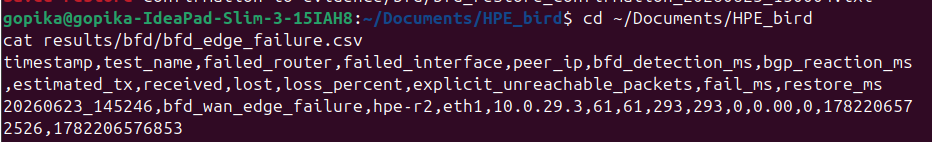
\includegraphics[width=0.95\textwidth]{../screenshots/bfd/01_bfd_detection_result_csv.png}
\caption{BFD detection result CSV}
\end{figure}

\begin{figure}[H]
\centering
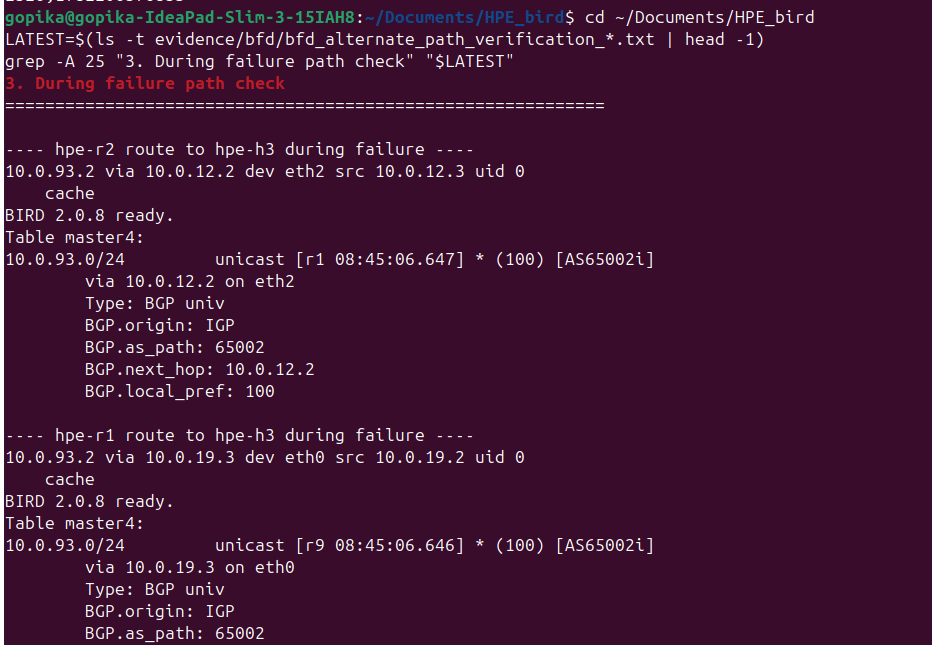
\includegraphics[width=0.95\textwidth]{../screenshots/bfd/02_bfd_alternate_path_during_failure.png}
\caption{BFD alternate path during failure}
\end{figure}

\begin{figure}[H]
\centering
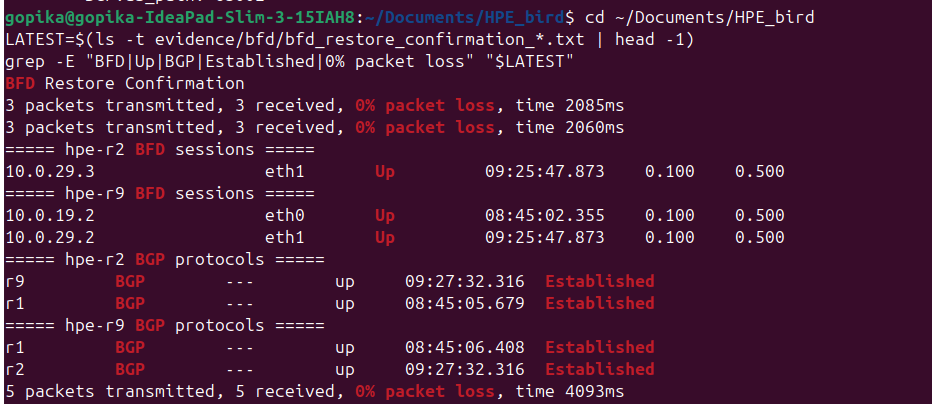
\includegraphics[width=0.95\textwidth]{../screenshots/bfd/03_bfd_restore_confirmation.png}
\caption{BFD restore confirmation}
\end{figure}

\begin{figure}[H]
\centering
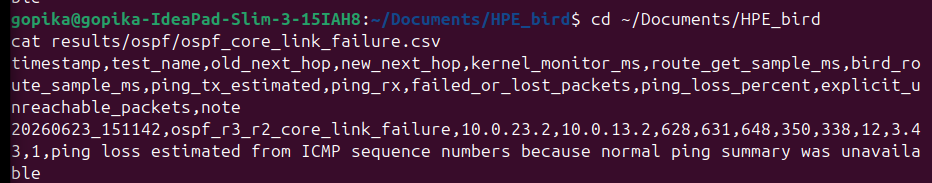
\includegraphics[width=0.95\textwidth]{../screenshots/ospf_core_failure/01_ospf_core_failure_csv.png}
\caption{OSPF core failure CSV}
\end{figure}

\begin{figure}[H]
\centering
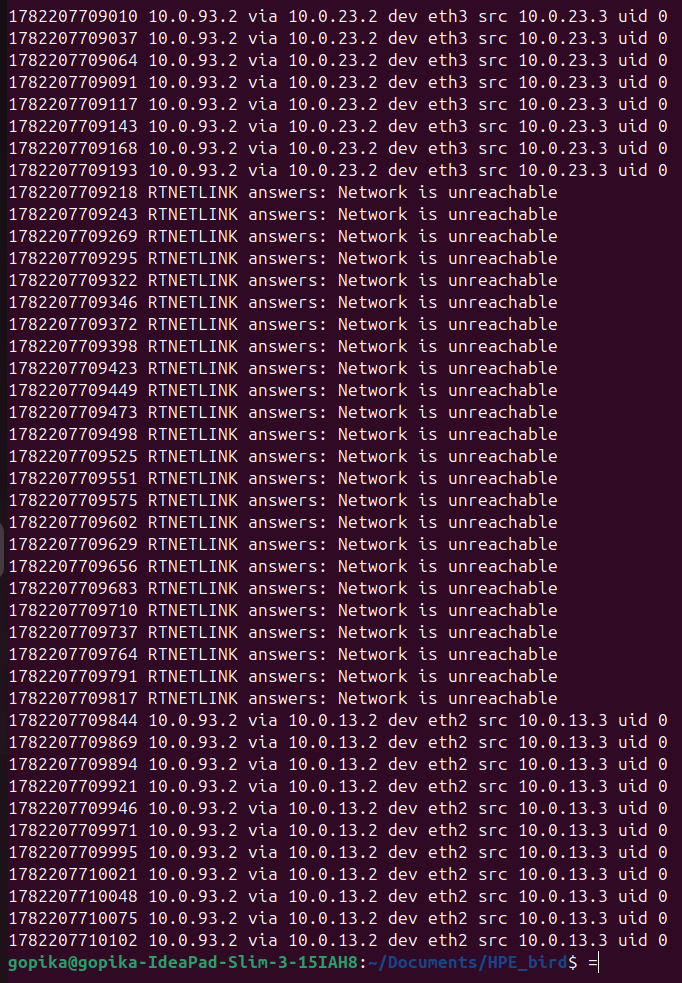
\includegraphics[width=0.95\textwidth]{../screenshots/ospf_core_failure/03_ospf_route_get_samples.png}
\caption{OSPF route sampling during recovery}
\end{figure}

\begin{figure}[H]
\centering
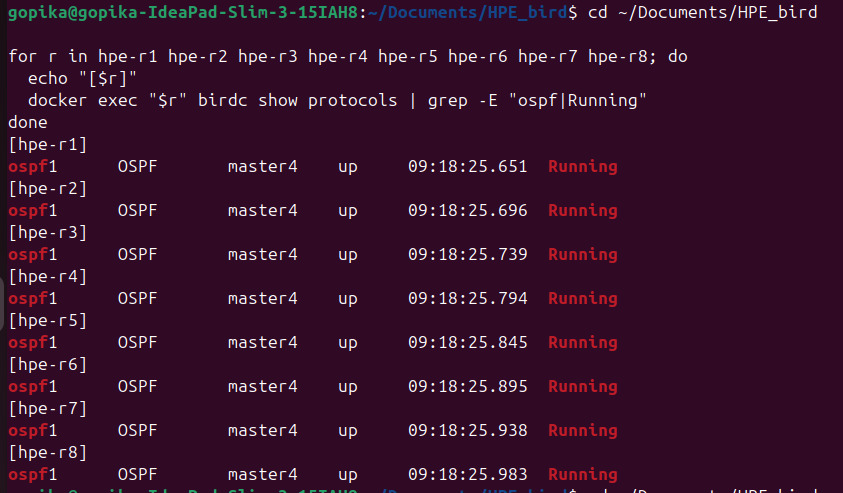
\includegraphics[width=0.95\textwidth]{../screenshots/ospf_core_failure/04_ospf_final_health.png}
\caption{OSPF final health}
\end{figure}

\begin{figure}[H]
\centering
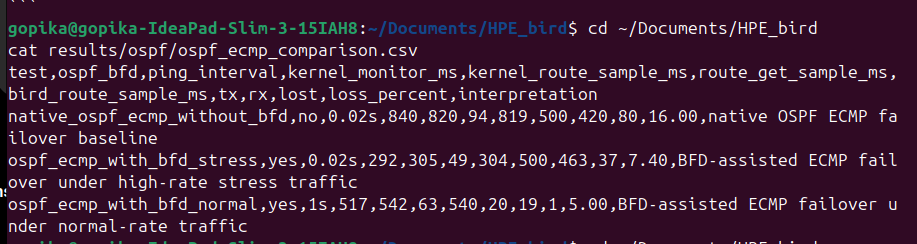
\includegraphics[width=0.95\textwidth]{../screenshots/ospf_ecmp/01_ospf_ecmp_comparison_csv.png}
\caption{OSPF ECMP comparison CSV}
\end{figure}

\begin{figure}[H]
\centering
\includegraphics[width=0.95\textwidth]{../screenshots/ospf_ecmp/02_ecmp_route_before_failure.png}
\caption{OSPF ECMP route before failure}
\end{figure}

\begin{figure}[H]
\centering
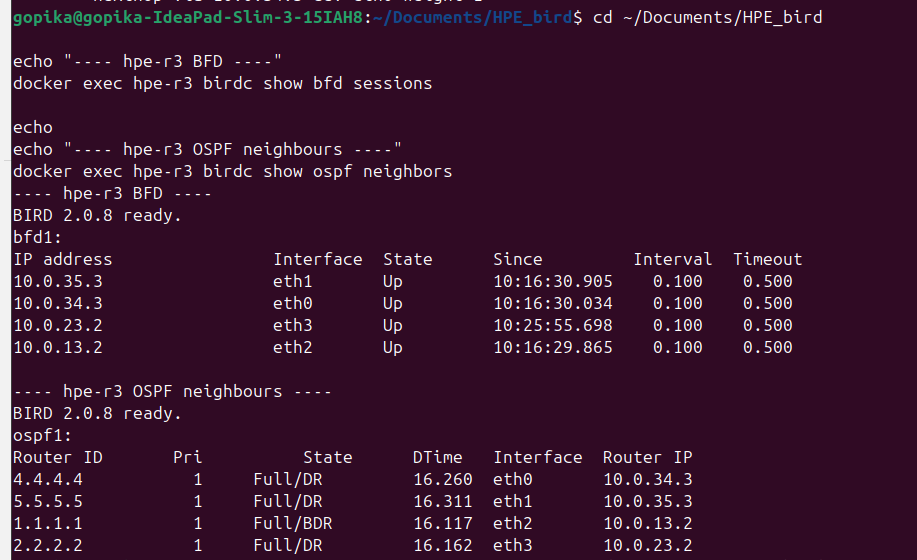
\includegraphics[width=0.95\textwidth]{../screenshots/ospf_ecmp/03_ospf_bfd_sessions_active.png}
\caption{OSPF-BFD sessions active}
\end{figure}

\begin{figure}[H]
\centering
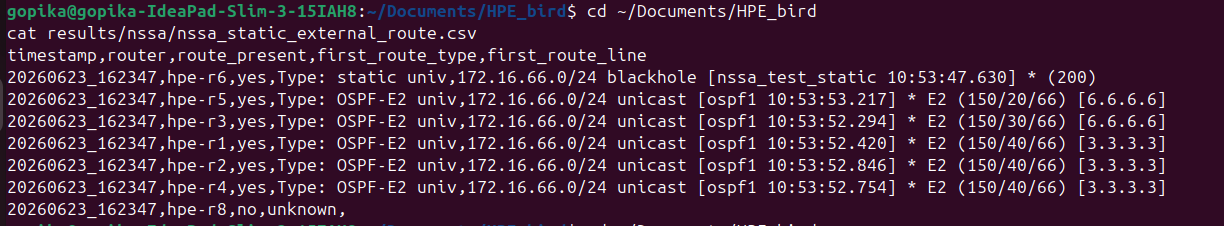
\includegraphics[width=0.95\textwidth]{../screenshots/nssa/01_nssa_type7_type5_csv.png}
\caption{NSSA Type-7 and Type-5 CSV}
\end{figure}

\begin{figure}[H]
\centering
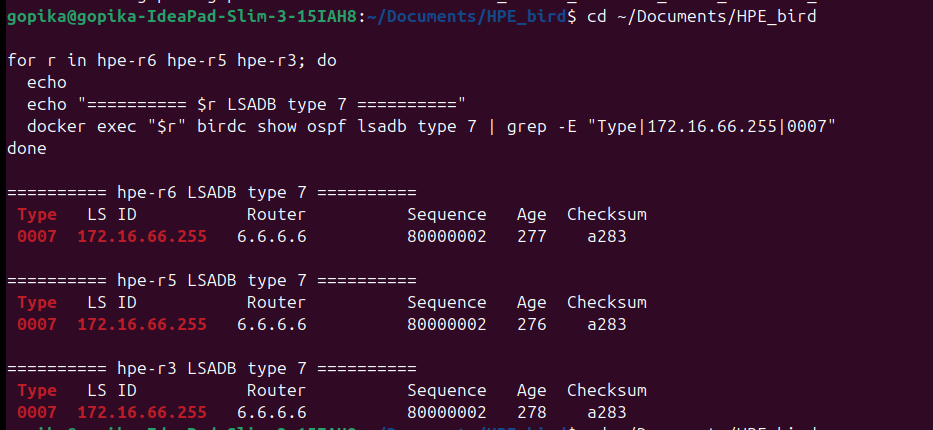
\includegraphics[width=0.95\textwidth]{../screenshots/nssa/02_type7_inside_nssa.png}
\caption{Type-7 LSA inside NSSA}
\end{figure}

\begin{figure}[H]
\centering
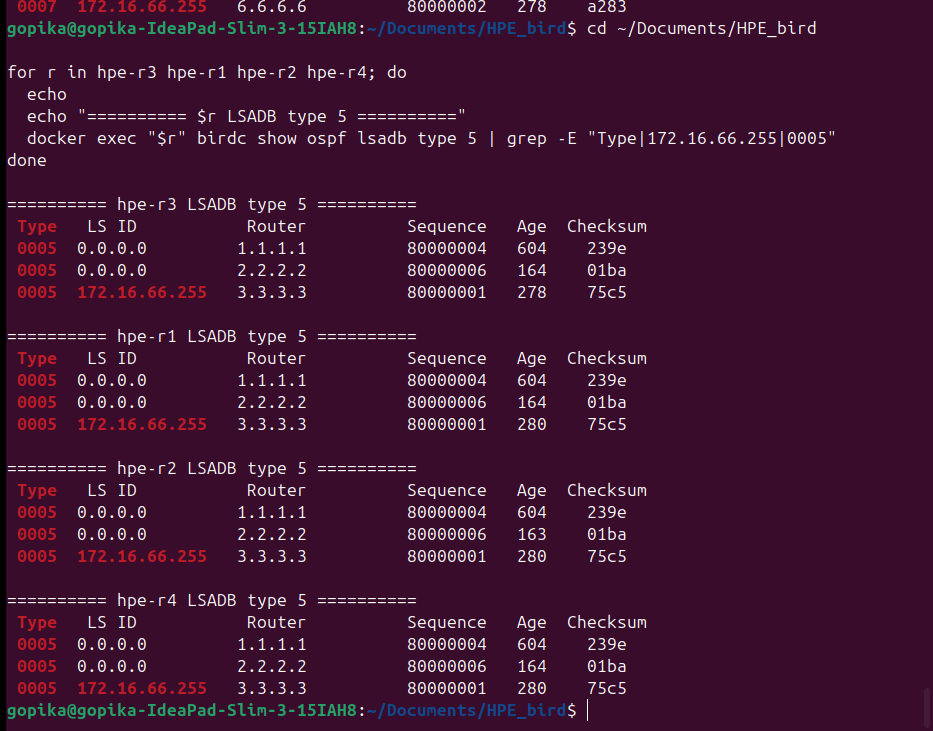
\includegraphics[width=0.95\textwidth]{../screenshots/nssa/03_type5_outside_nssa.png}
\caption{Type-5 LSA outside NSSA}
\end{figure}

\begin{figure}[H]
\centering
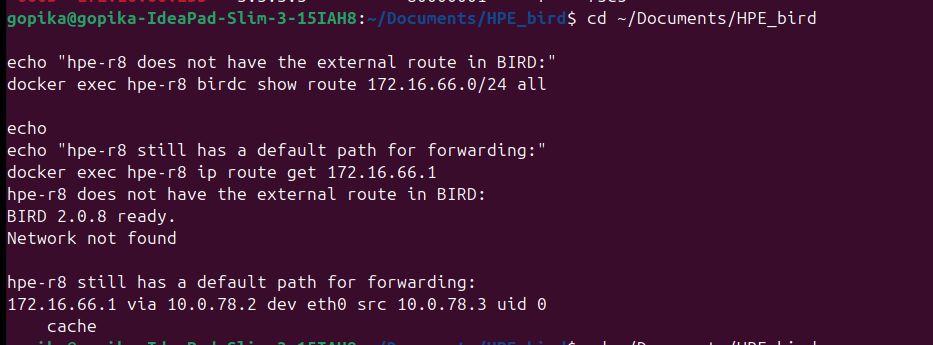
\includegraphics[width=0.95\textwidth]{../screenshots/nssa/04_stub_area_external_route_containment.png}
\caption{Stub area external route containment}
\end{figure}

\begin{figure}[H]
\centering
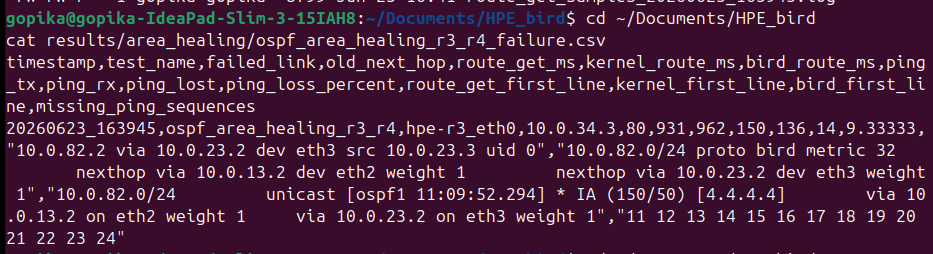
\includegraphics[width=0.95\textwidth]{../screenshots/area_healing/01_area_healing_csv.png}
\caption{OSPF area healing CSV}
\end{figure}

\begin{figure}[H]
\centering
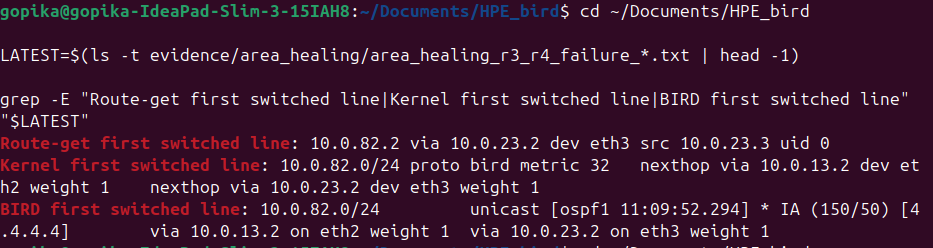
\includegraphics[width=0.95\textwidth]{../screenshots/area_healing/03_route_after_healing.png}
\caption{OSPF area route after healing}
\end{figure}

\begin{figure}[H]
\centering
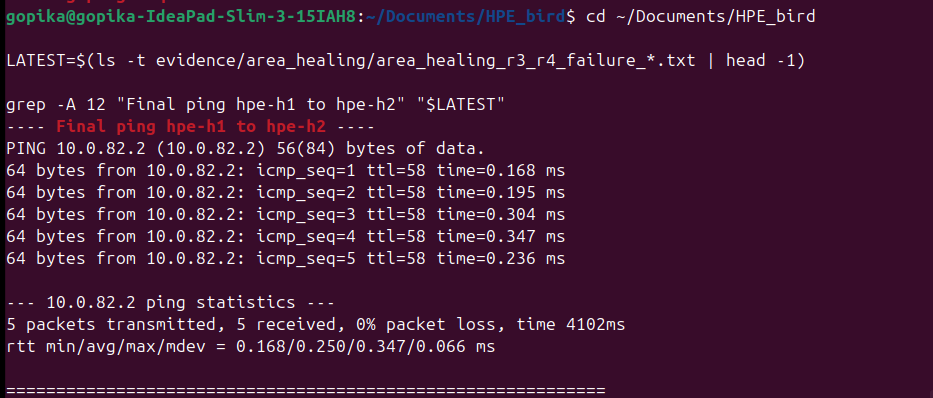
\includegraphics[width=0.95\textwidth]{../screenshots/area_healing/05_final_restored_health.png}
\caption{OSPF area final restored health}
\end{figure}

\begin{figure}[H]
\centering
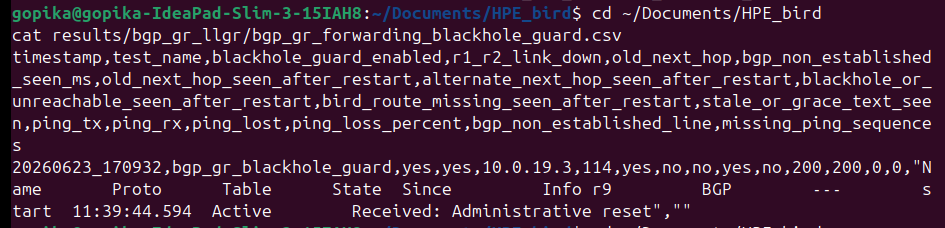
\includegraphics[width=0.95\textwidth]{../screenshots/bgp_gr_llgr/01_bgp_gr_blackhole_guard_csv.png}
\caption{BGP GR blackhole guard CSV}
\end{figure}

\begin{figure}[H]
\centering
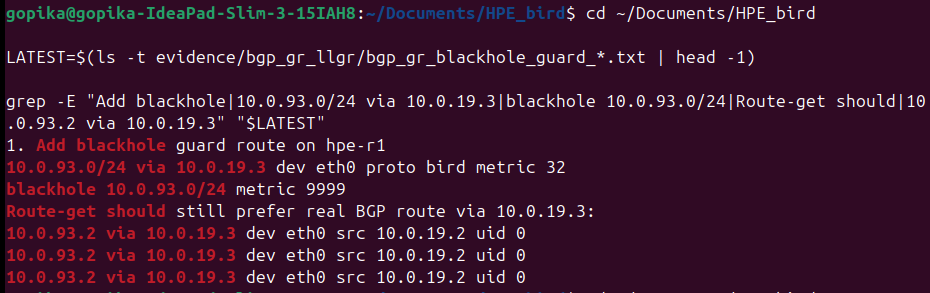
\includegraphics[width=0.95\textwidth]{../screenshots/bgp_gr_llgr/02_blackhole_guard_real_route_preferred.png}
\caption{BGP GR blackhole guard real route preferred}
\end{figure}

\begin{figure}[H]
\centering
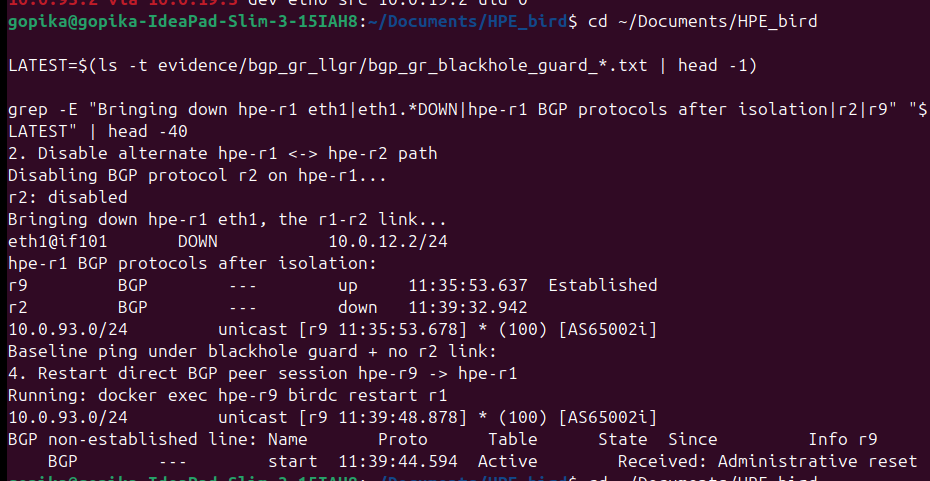
\includegraphics[width=0.95\textwidth]{../screenshots/bgp_gr_llgr/03_alternate_path_disabled.png}
\caption{BGP alternate path disabled}
\end{figure}

\begin{figure}[H]
\centering
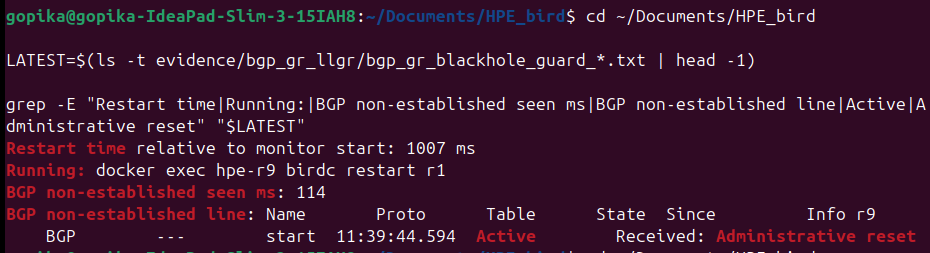
\includegraphics[width=0.95\textwidth]{../screenshots/bgp_gr_llgr/04_bgp_restart_observed.png}
\caption{BGP restart observed}
\end{figure}

\begin{figure}[H]
\centering
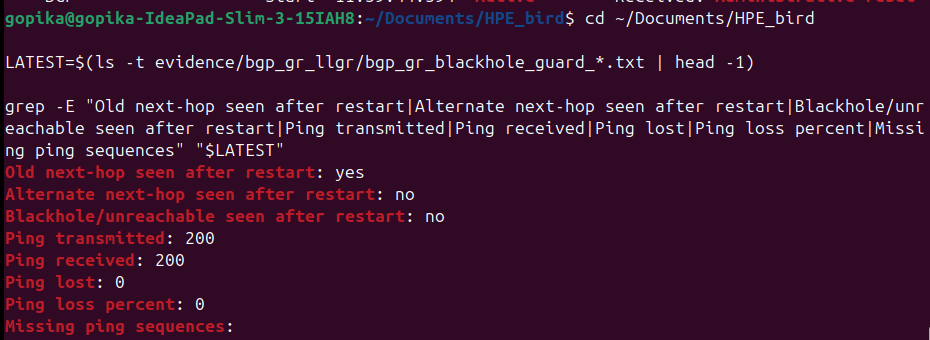
\includegraphics[width=0.95\textwidth]{../screenshots/bgp_gr_llgr/05_forwarding_continued_no_fallback.png}
\caption{BGP forwarding continued without fallback}
\end{figure}

\begin{figure}[H]
\centering
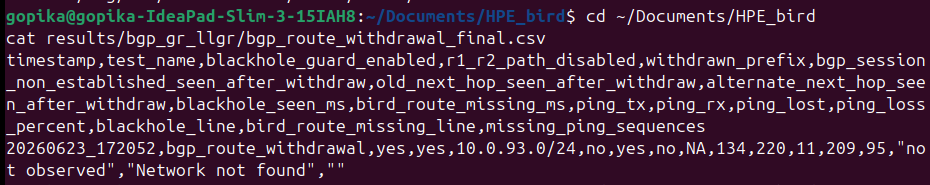
\includegraphics[width=0.95\textwidth]{../screenshots/bgp_gr_llgr/06_bgp_withdrawal_csv.png}
\caption{BGP withdrawal CSV}
\end{figure}

\begin{figure}[H]
\centering
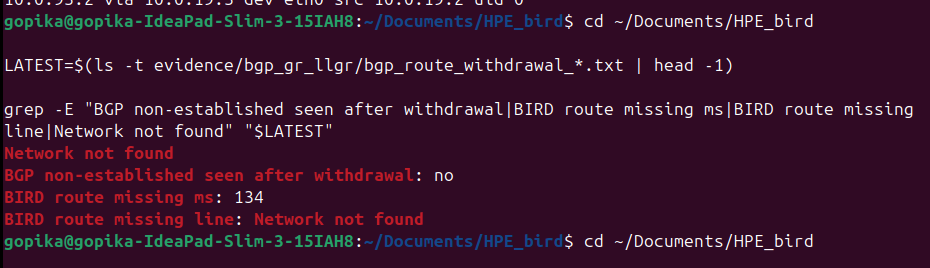
\includegraphics[width=0.95\textwidth]{../screenshots/bgp_gr_llgr/08_route_withdrawn_bgp_still_up.png}
\caption{BGP route withdrawn while session stayed up}
\end{figure}

\begin{figure}[H]
\centering
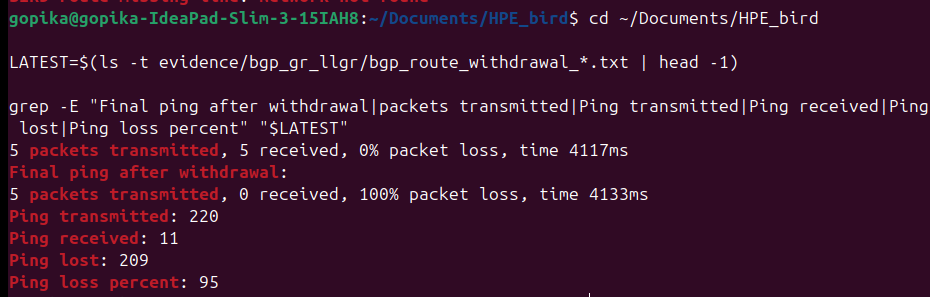
\includegraphics[width=0.95\textwidth]{../screenshots/bgp_gr_llgr/09_withdrawal_packet_loss.png}
\caption{BGP withdrawal packet loss}
\end{figure}

% --- NEW DELIVERABLE TERMINAL SCREENSHOTS START ---

\subsection{Additional Deliverable Terminal Evidence}

The following screenshots show terminal evidence for the additional deliverable experiments: multi-hop BFD, BGP full daemon restart, and BGP peer flap recovery.

\begin{figure}[H]
\centering
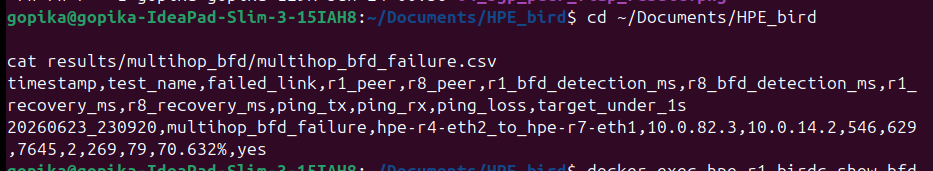
\includegraphics[width=0.95\textwidth]{../screenshots/new_deliverables_terminal/01_multihop_bfd_sessions.png}
\caption{01 multihop bfd sessions}
\end{figure}

\begin{figure}[H]
\centering
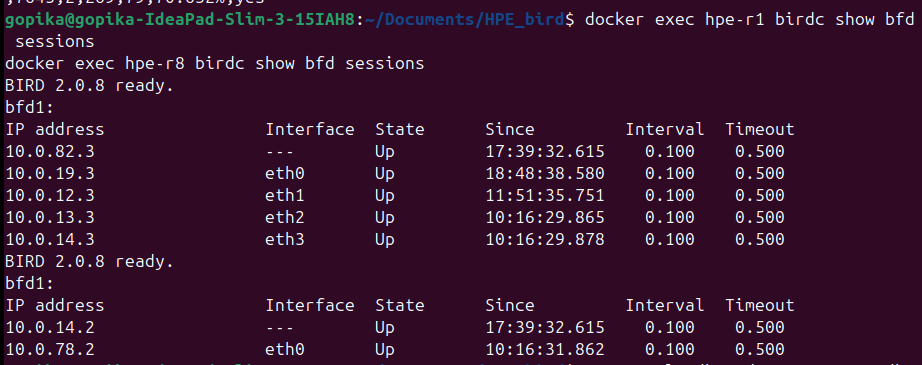
\includegraphics[width=0.95\textwidth]{../screenshots/new_deliverables_terminal/02_multihop_bfd_result_csv.png}
\caption{02 multihop bfd result csv}
\end{figure}

\begin{figure}[H]
\centering
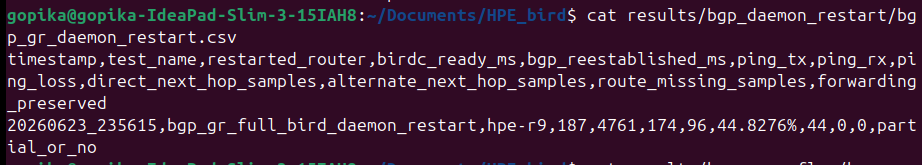
\includegraphics[width=0.95\textwidth]{../screenshots/new_deliverables_terminal/03_bgp_daemon_restart_result_csv.png}
\caption{03 bgp daemon restart result csv}
\end{figure}

\begin{figure}[H]
\centering
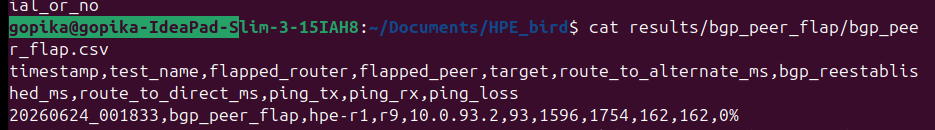
\includegraphics[width=0.95\textwidth]{../screenshots/new_deliverables_terminal/04_bgp_peer_flap_result_csv.png}
\caption{04 bgp peer flap result csv}
\end{figure}

% --- NEW DELIVERABLE TERMINAL SCREENSHOTS END ---

\begin{figure}[H]
\centering
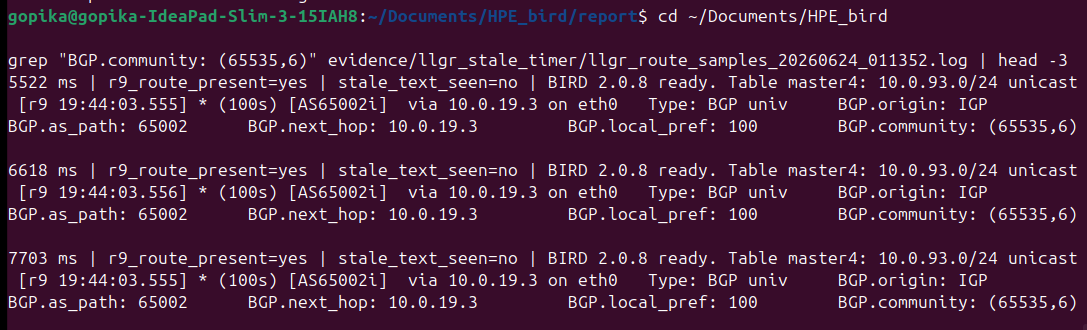
\includegraphics[width=0.95\textwidth]{../screenshots/new_deliverables_terminal/05_llgr_stale_marker.png}
\caption{LLGR stale route marker shown as \texttt{(100s)} and \texttt{BGP.community: (65535,6)}}
\end{figure}




\end{document}
